%% 
%% Copyright 2007-2025 Elsevier Ltd
%% 
%% This file is part of the 'Elsarticle Bundle'.
%% ---------------------------------------------
%% 
%% It may be distributed under the conditions of the LaTeX Project Public
%% License, either version 1.3 of this license or (at your option) any
%% later version.  The latest version of this license is in
%%    http://www.latex-project.org/lppl.txt
%% and version 1.3 or later is part of all distributions of LaTeX
%% version 1999/12/01 or later.
%% 
%% The list of all files belonging to the 'Elsarticle Bundle' is
%% given in the file `manifest.txt'.
%% 
%% Template article for Elsevier's document class `elsarticle'
%% with numbered style bibliographic references
%% SP 2008/03/01
%% $Id: elsarticle-template-num.tex 272 2025-01-09 17:36:26Z rishi $
%%
%\documentclass[preprint,12pt]{elsarticle}

%% Use the option review to obtain double line spacing
%% \documentclass[authoryear,preprint,review,12pt]{elsarticle}

%% Use the options 1p,twocolumn; 3p; 3p,twocolumn; 5p; or 5p,twocolumn
%% for a journal layout:
\documentclass[final,1p,times]{elsarticle}
%% \documentclass[final,1p,times,twocolumn]{elsarticle}
%% \documentclass[final,3p,times]{elsarticle}
%% \documentclass[final,3p,times,twocolumn]{elsarticle}
%% \documentclass[final,5p,times]{elsarticle}
%% \documentclass[final,5p,times,twocolumn]{elsarticle}

%% For including figures, graphicx.sty has been loaded in
%% elsarticle.cls. If you prefer to use the old commands
%% please give \usepackage{epsfig}

%% The amssymb package provides various useful mathematical symbols
\usepackage{amssymb}
%% The amsmath package provides various useful equation environments.
\usepackage{amsmath}
%% The amsthm package provides extended theorem environments
%% \usepackage{amsthm}
\usepackage{hyperref}

% User-added packages
\usepackage{listings}
\usepackage{array}
\usepackage{xcolor}
\usepackage{soul}
\usepackage{booktabs}
%\usepackage{manyfoot}%
%\usepackage{footnote}
%\makesavenoteenv{tabular}  % if using footnotes inside tabular
\usepackage{tabularx}
\usepackage{geometry}
\usepackage{threeparttable}
\usepackage[nolist]{acronym}
\usepackage[figuresright]{rotating} % include this in your preamble
\usepackage{adjustbox}
\usepackage{tablefootnote}

% Define a muted color palette
\definecolor{codebg}{RGB}{253, 253, 253}
\definecolor{keywordcolor}{RGB}{30,60,114}
\definecolor{stringcolor}{RGB}{50,100,50}
\definecolor{commentcolor}{RGB}{150,150,150}
\definecolor{identifiercolor}{RGB}{40,40,40}
\definecolor{codegreen}{rgb}{0,0.6,0}
\definecolor{codegray}{rgb}{0.5,0.5,0.5}
\definecolor{codepurple}{rgb}{0.58,0,0.82}
\definecolor{backcolour}{rgb}{0.95,0.95,0.92}
\definecolor{darkred}{rgb}{0.6,0.0,0.0}
\definecolor{darkgreen}{rgb}{0,0.50,0}
\definecolor{lightblue}{rgb}{0.0,0.42,0.91}
\definecolor{orange}{rgb}{0.99,0.48,0.13}
\definecolor{grass}{rgb}{0.18,0.80,0.18}
\definecolor{pink}{rgb}{0.97,0.15,0.45}

% Custom command definitions
%\newcommand*{\figref}[2][]{%
%  \hyperref[{#2}]{%
%    \ref*{#2}%
%    \ifx\\#1\\%
%    \else
%      #1%
%    \fi
%  }%
%}

% General Setting of listings
\lstset{
  aboveskip=1em,
  breaklines=true,
  abovecaptionskip=6pt,
  captionpos=b,
  escapeinside={\%*}{*)},
  frame=single,
  numbers=left,
  numbersep=10pt,
  tabsize=2,
  keepspaces=true,                                    
  showspaces=false,                
  showstringspaces=false,
  showtabs=false,
  numberstyle=\tiny,
  breakatwhitespace=false,         
  breaklines=true,
  basicstyle=\ttfamily, %\footnotesize
}
% 1. General Python Keywords List
\lstdefinelanguage{PythonReemission}[]{Python}{
  morekeywords=[1]{,as,assert,nonlocal,with,yield,self,True,False,None,} % Python builtin
  morekeywords=[2]{,__init__,__add__,__mul__,__div__,__sub__,__call__,__getitem__,__setitem__,__eq__,__ne__,__nonzero__,__rmul__,__radd__,__repr__,__str__,__get__,__truediv__,__pow__,__name__,__future__,__all__,}, % magic methods
  morekeywords=[3]{,object,type,isinstance,copy,deepcopy,zip,enumerate,reversed,list,set,len,dict,tuple,range,xrange,append,execfile,real,imag,reduce,str,repr,}, % common functions
  morekeywords=[4]{,Exception,NameError,IndexError,SyntaxError,TypeError,ValueError,OverflowError,ZeroDivisionError,}, % errors
  morekeywords=[5]{,ode,fsolve,sqrt,exp,sin,cos,arctan,arctan2,arccos,pi, array,norm,solve,dot,arange,isscalar,max,sum,flatten,shape,reshape,find,any,all,abs,plot,linspace,legend,quad,polyval,polyfit,hstack,concatenate,vstack,column_stack,empty,zeros,ones,rand,vander,grid,pcolor,eig,eigs,eigvals,svd,qr,tan,det,logspace,roll,min,mean,cumsum,cumprod,diff,vectorize,lstsq,cla,eye,xlabel,ylabel,squeeze,},
  emph={,ReemissionEngine, MonthlyTemperature, CarbonDioxideEmission, NitrousOxideEmission, MethaneEmission, Landuse, Climate, SoilType, Biome, TreatmentFactor, LanduseIntensity, Catchment, Reservoir, BiogenicFactors}, % numpy / math
}

% 3. Extended theme
\lstdefinestyle{colorEX}{
  basicstyle=\ttfamily\footnotesize,
  backgroundcolor=\color{codebg},
  commentstyle=\color{darkgreen}\slshape,
  keywordstyle=\color{blue}\bfseries\itshape,
  keywordstyle=[2]\color{blue}\bfseries,
  keywordstyle=[3]\color{grass},
  keywordstyle=[4]\color{red},
  keywordstyle=[5]\color{orange},
  stringstyle=\color{darkred},
  emphstyle=\color{pink}\underbar,
  numberstyle=\tiny\color{codegray},
  numbersep=10pt,
}
\lstdefinestyle{custmpythonstyle}{
    backgroundcolor=\color{codebg},
    commentstyle=\color{commentcolor}\itshape,
    keywordstyle=\color{keywordcolor}\bfseries,
    stringstyle=\color{stringcolor},
    identifierstyle=\color{identifiercolor},
    breaklines=true,
    captionpos=b,
    keepspaces=true,
    numbers=left,
    frame=single,
    numbersep=10pt,
    rulecolor=\color{gray},
    showstringspaces=false
}

\lstdefinelanguage{Dockerfile}{
  morekeywords={FROM, RUN, CMD, LABEL, MAINTAINER, EXPOSE, ENV, ADD, COPY, ENTRYPOINT, VOLUME, USER, WORKDIR, ARG, ONBUILD, STOPSIGNAL, HEALTHCHECK, SHELL},
  sensitive=true,
  morecomment=[l]{\#},
  morestring=[b]"
}

\lstset{style=colorEX}

%% The lineno packages adds line numbers. Start line numbering with
%% \begin{linenumbers}, end it with \end{linenumbers}. Or switch it on
%% for the whole article with \linenumbers.
%% \usepackage{lineno}

\usepackage{caption}
\captionsetup[lstlisting]{font=small}
\captionsetup[table]{font=normalsize}
\captionsetup[figure]{font=normalsize}
\captionsetup[bibliography]{font=normalsize}

\usepackage[linesnumbered,ruled,vlined]{algorithm2e}

\usepackage{refcount}  % for \getrefnumber
\usepackage{xparse}    % for optional arguments
\NewDocumentCommand{\figref}{O{}m}{%
  \hyperref[#2]{\ref*{#2}#1}%
}

%\NewDocumentCommand{\figref}{O{}m}{%
%  \getrefnumber{#2}#1%
%}

% This will be executed when \appendix is called
\AtBeginDocument{%
  \let\oldappendix\appendix
  \renewcommand{\appendix}{%
    \oldappendix
    % Reset counters
    \setcounter{figure}{0}
    \setcounter{table}{0}
    \setcounter{equation}{0}
    \setcounter{lstlisting}{0}
    
    % Redefine the counter representation
    \renewcommand{\thefigure}{A.\arabic{figure}}
    \renewcommand{\thetable}{A.\arabic{table}}
    \renewcommand{\theequation}{A.\arabic{equation}}
    \renewcommand{\thelstlisting}{A.\arabic{lstlisting}}
  }
}

\makeatletter
\newcommand{\vrbbrk}[1]{%
  \begingroup
  \ttfamily
  \begingroup\lccode`~=`/\lowercase{\endgroup\def~}{/\discretionary{}{}{}}%
  \begingroup\lccode`~=`[\lowercase{\endgroup\def~}{[\discretionary{}{}{}}%
  \begingroup\lccode`~=`.\lowercase{\endgroup\def~}{.\discretionary{}{}{}}%
  \catcode`/=\active\catcode`[=\active\catcode`.=\active
  \scantokens{#1\noexpand}%
  \endgroup
}
\makeatother


\journal{Environmental Modelling \& Software}

\begin{document}

\begin{frontmatter}

%% Title, authors and addresses

%% use the tnoteref command within \title for footnotes;
%% use the tnotetext command for theassociated footnote;
%% use the fnref command within \author or \affiliation for footnotes;
%% use the fntext command for theassociated footnote;
%% use the corref command within \author for corresponding author footnotes;
%% use the cortext command for theassociated footnote;
%% use the ead command for the email address,
%% and the form \ead[url] for the home page:
%% \title{Title\tnoteref{label1}}
%% \tnotetext[label1]{}
%% \author{Name\corref{cor1}\fnref{label2}}
%% \ead{email address}
%% \ead[url]{home page}
%% \fntext[label2]{}
%% \cortext[cor1]{}
%% \affiliation{organization={},
%%             addressline={},
%%             city={},
%%             postcode={},
%%             state={},
%%             country={}}
%% \fntext[label3]{}

\title{\emph{Re-Emission} - A free open-source software for estimating, reporting and visualizing greenhouse gas emissions from reservoirs}

%% use optional labels to link authors explicitly to addresses:
 \author[label1]{Tomasz Janus}
 \affiliation[label1]{organization={Tyndall Centre Manchester, University of Manchester},
             addressline={Floor 5, Engineering A, Booth Street East},
             city={Manchester},
             postcode={M13 9PL},
             %state={},
             country={United Kingdom}}
 \author[label2]{Christopher Barry}
 \affiliation[label2]{organization={UK Centre for Ecology \& Hydrology},
             addressline={Deiniol Road},
             city={Bangor},
             postcode={LL57 2UW},
             %state={},
             country={United Kingdom}}           
 \author[label3,label4]{Xingxing Zhang}
 \affiliation[label3]{organization={State Key Laboratory of Resources and Environmental Information System, Institute of Geographic Sciences and Natural Resources Research},
             addressline={Chinese Academy of Sciences},
             city={Beijing},
             %postcode={M13 9PL},
             %state={},
             country={China}}
 \affiliation[label4]{organization={College of Resources and Environment},
             addressline={University of Chinese Academy of Sciences},
             city={Beijing},
             %postcode={M13 9PL},
             %state={},
             country={China}} 
 \author[label1]{Jaise Kuriakose}           

%% Abstract
\begin{abstract}
%Reservoirs collectively contribute approximately 1-2\% of total anthropogenic greenhouse gas emissions.
%These broad impacts on the atmosphere and climate should be appropriately assessed and reported.
Reservoirs are significant contributors to anthropogenic \ac{GHG} emissions whose broad impacts on the climate should be appropriately assessed and reported. 
Yet, existing tools for estimating reservoir emissions are limited in their application, or require extensive data inputs which requires significant manual effort limiting their application to small numbers of reservoirs.
Here, we present an open-source tool, \emph{Re-Emission}, which simplifies and streamlines reservoir emission modelling and enables estimation of emissions from regional and national scale reservoir inventories. 
%The software can be extended with new modules; these may pertain to \ac{GHG} emissions estimation, but also other aspects of landscape-aquatic bio-geochemistry.
We demonstrate the utility of our software on two practical case studies estimating emissions from $\sim$250 reservoirs.
Our tool can be introduced into larger multi-domain frameworks to enable the use of reservoir emissions to support decision-making -- for example in water resources and energy planning.
It integrates with a catchment analysis tool to provide automated reservoir emission assessments, removing the need for extensive user input -- a key barrier to a broader adoption of spatially-explicit emission models.
%energy policy and hydropower development, especially in tropical regions, where the climate benefits of hydropower may be substantially less than previously assumed
\end{abstract}

%%Graphical abstract
\begin{graphicalabstract}
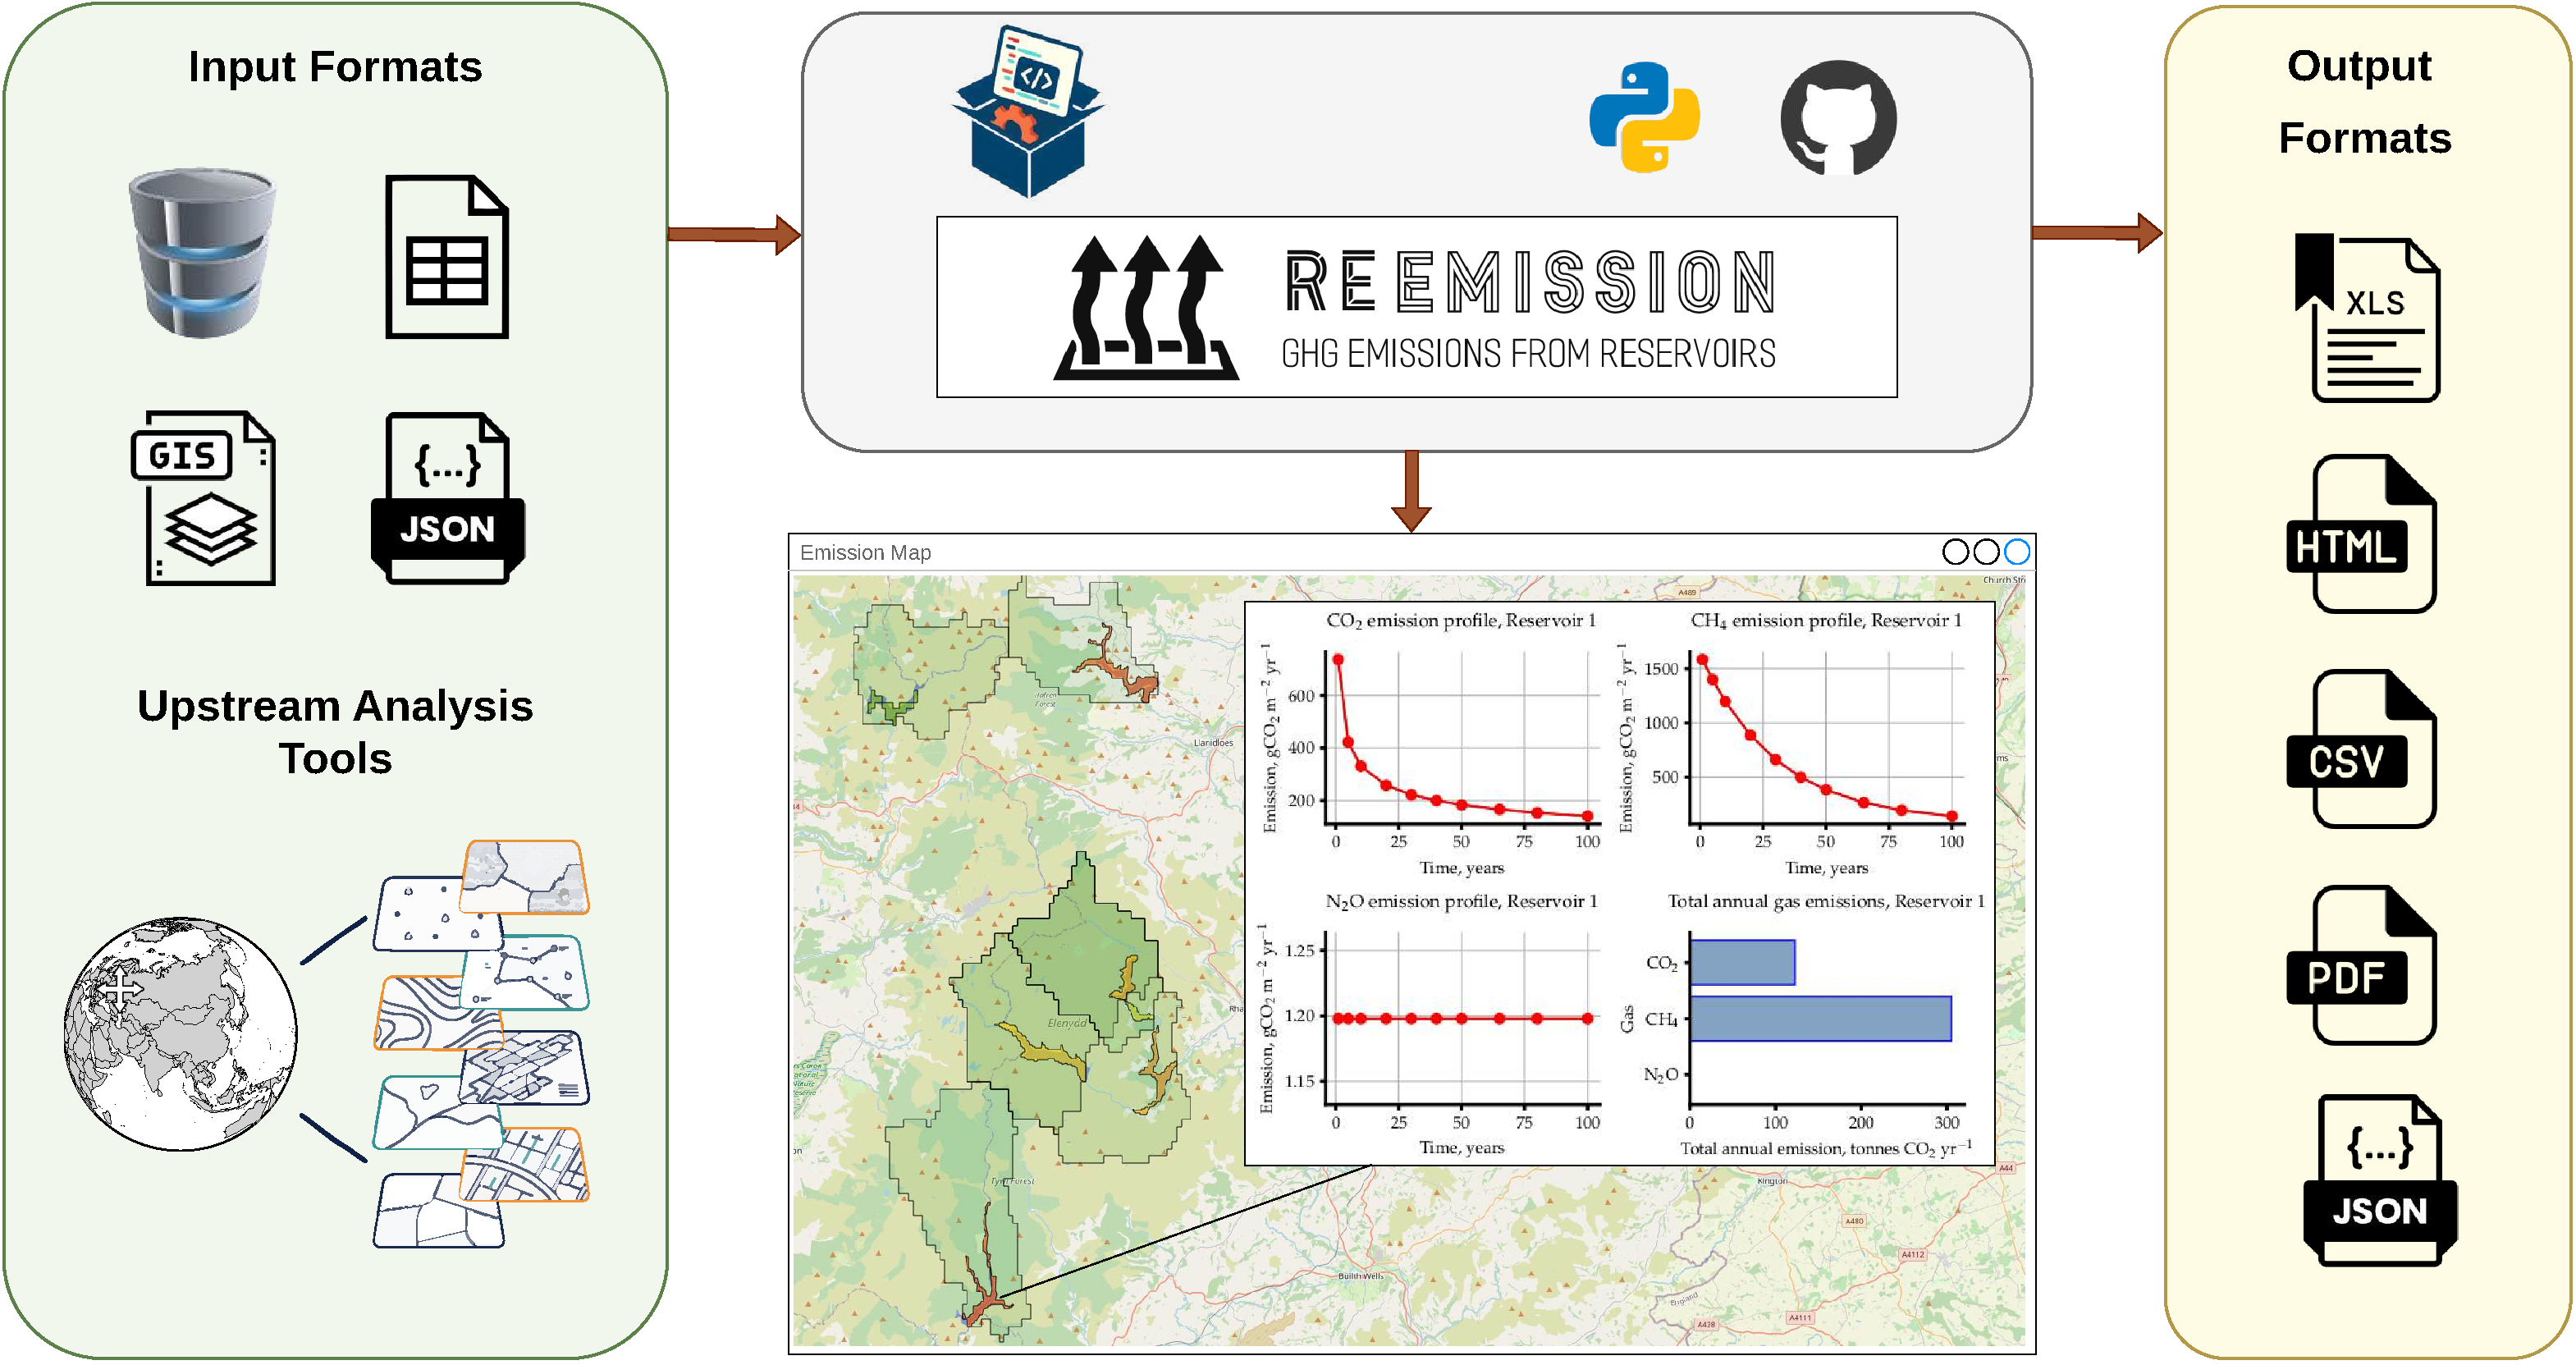
\includegraphics[width=1\textwidth]{figures/graphical_abstract_new.drawio-compressed.pdf}
\end{graphicalabstract}

%%Research highlights
\begin{highlights}
\item Command line tool and a Python library for calculating reservoir emissions.
\item Configurable calculation and visualization options.
\item Integrates with \acs{GIS}-based catchment and reservoir delineation tool.
%\item Automates emission calculations from multiple reservoirs.
\item Supports multiple output and report formats.
\item Applications in the United Kingdom and Myanmar highlight Re-Emission's features.
\end{highlights}

%% Keywords
\begin{keyword}
automated assessments \sep greenhouse gas emissions \sep reservoirs \sep open source
%% keywords here, in the form: keyword \sep keyword
%% PACS codes here, in the form: \PACS code \sep code
%% MSC codes here, in the form: \MSC code \sep code
%% or \MSC[2008] code \sep code (2000 is the default)
\end{keyword}

\end{frontmatter}

\section{Introduction}
\label{sec:introduction}

Reservoirs are increasingly recognized as significant sources of biogenic \ac{GHG} emissions~\citep{Barros2011}, particularly in low-altitude tropical regions, where emission intensities (e.g., kg~CO$_{2e}$\,MWh$^{-1}$) of hydroelectric dams might exceed those of fossil fuel power plants~\citep{Fearnside2002}.
The emissions arise from the decomposition of organic matter that was flooded during reservoir construction, transferred to the reservoir by river run-off, or grown in the reservoir such as by algal production~\citep{Louis2000}.
Most recent estimates put their contribution globally at approximately 5.2\% of total anthropogenic \ac{CH4} emissions and 0.2\% of \ac{CO2} emissions; together equivalent to 1-2\% of total anthropogenic \ac{GHG} emissions~\cite{Soued2022}.
The ongoing and planned investments in reservoir infrastructure worldwide are likely to hamper efforts to meet the Paris global climate change targets.
In the hydroelectric sector alone, more than 3,700 dams are planned~\cite{Zarfl2015,Bouckaert2021} that could contribute approximately 400\,MtCO$_{2e}$ to global emissions annually~\cite{janus2025planning} -- equivalent to circa 11\% of the EU’s emissions. 
Projections for planned reservoir investments from other sectors such as flood control and water supply are less known but likely to be substantial, due to a pressing need to close the growing water storage gap \cite{Yu2021} and improve the resilience of water resource systems to climatic uncertainty~\cite{ipcc2018, Sarkodie2022}.
Given the potentially high \ac{GHG} fluxes (areal emissions) from reservoirs, rigorous estimation of emissions is needed (i) from planned reservoirs to design optimal low-carbon optimal expansion strategies and (ii) from existing reservoirs to provide more accurate estimates of the contribution of reservoir emissions to global emissions.

%Although several estimates of the total number and total area of reservoirs worldwide have been constructed, contemporary advances in remote sensing and global hydrological mapping have considerably increased our understanding of their true extent and distribution.
%\citet{Downing2006} estimated the number of impoundments globally at 515,149 with a total area of 258,570~km$^2$
%More recent studies provide significantly higher estimates: $\sim$2.8 million reservoirs with a total area of $\sim$530,000~km$^2$~\cite{Mulligan2020} and $\sim$2.5 million with $\sim$642,000~km$^2$ total surface area~\cite{LehnerMessager2023}. 
%All of the above figures are considerably larger than those reported in global dam databases such as \acs{FHReD}~\cite{Zarfl2015FHReD} ($\sim$40,000), \acs{GOOD2}~\cite{Mulligan2021GOOD2} ($\sim$38,667), or \acs{ICOLD}~\cite{ICOLD2020} ($\sim$58,700). 
%These discrepancies stem largely from improved satellite imagery and detection methods that can now identify millions of small and previously undocumented reservoirs.
%Given the likely exclusion of numerous existing reservoirs with unquantified atmospheric impacts, current global emission estimates may require reassessment to account for these new contributions.

Several studies have addressed the methodological challenges of quantifying reservoir emissions and have provided estimates of \ac{GHG} emissions from existing reservoirs at both global~\citep{Barros2011, Soued2022, Deemer2016, Prairie2018, Harrison2021} and regional scales~\citep{Hidrovo2017, Rasanen2018, Almeida2019, Hansen2022}. 
These studies have shown that emissions are shaped by a multitude of hydro-morphological, edaphic, climatic, and land-use characteristics of reservoirs and their catchments~\citep{Deemer2016, Prairie2021}.
%, thereby necessitating the use of comprehensive emission models for accurate site-specific assessments. 
Nevertheless, current global estimates, including the most recent~\citep{Harrison2021, Soued2022} relied on empirical flux approximations derived from a limited number of measured sites, rather than on application of spatially explicit emission models to individual reservoirs to individual reservoirs. 
Such approaches cannot capture the variability in emission fluxes driven by site-specific environmental conditions and reservoir properties~\cite{janus2025planning}, which in turns might impair the reliability of global assessments 
%(e.g.,~\citep{Harrison2021, Soued2022})
and strategic planning efforts. % (e.g.,~\cite{Almeida2019, Carlino2024, Tangi2024}).
Moreover, the underlying measurement data used for upscaling tend to be skewed toward large, deep, hydroelectric reservoirs~\cite{Hansen2022}, thereby underrepresenting small reservoirs~\citep{Malerba2022} which are often shallow, and typically rich in organic matter -- conditions that are conducive to elevated methane production~\citep{WANG2025123441, SHI2025}. 
Hence, the global \acp{EF} derived in recent assessments~\citep{Harrison2021, Soued2022} might underestimate emissions from small, shallow reservoirs, such as those used for irrigation and introduce biases into global reservoir assessments.

A major barrier to addressing the challenges outlined above is the lack of software capable of estimating reservoir emissions at national, regional, and global scales using the most up-to-date emission models that go beyond Tier~1 \acf{EF} approaches and basic upscaling techniques.
The most comprehensive and widely recognized model for estimating reservoir \ac{GHG} emissions is the G-res model~\cite{Prairie2017b, Prairie2021}, which provides spatially explicit estimates of gross and net emissions by accounting for both anthropogenic and natural sources, as well as a wide range of climatic, hydro-morphological, edaphic, and land-use drivers.
The model is supported by a publicly available web-based platform, the G-res Tool~\cite{prairie2017gres}, which offers free emission assessments for non-commercial users and a paid service for commercial applications.
However, the G-res Tool is primarily intended for single-reservoir assessments and lacks functionality for large-scale or batch analyses.
It requires considerable manual effort to input site-specific data, and as a web-based platform with a fixed interface, it cannot be readily automated for large-scale assessments involving multiple reservoirs.
Furthermore, the tool is closed-source and offers limited potential for customization.
As such, it is not well-suited for advanced applications such as stochastic modelling, strategic planning, or extensions that incorporate custom emission models.

%The development of a free open-source alternative could offer the following benefits: (i) direct use of complete emission models, instead of upscaling methods, may help removing potential biases in global estimates and improve the accuracy of emission estimates for individual reservoirs, (ii) they will enable a more precise estimation of emissions from reservoirs whose characteristics fall outside the range of values represented in the measurement data sets (iii) they will enable an easier transition from Tier~1 may not be adequate to represent emission rates in different regions as well as different reservoir morphologies into more methodological methods without imposing significant overheads in terms of costs and time, (iv) 

%This upscaling approach assumes that areal fluxes for a given gas or emission pathway remain constant within a specific area of interest, such as a latitude~\cite{Harrison2021} or climatic zone~\cite{Soued2022} and does not take into account the effects of the multitude of emission drivers on emission rates~\citep{Deemer2016, Prairie2021} that vary widely across the diverse reservoir morphologies and their geographic settings.
%upscaling emissions from a small number of reservoirs with measured emissions to global emissions by 
%Precision due to identification of reservoir area and locations and estimation methods - ever growing numbers 
%However, these databases a rather high estimate for total area\,km$^2$ -- ~480,000 in GOOD2.
%Shows that missing data is for small reservoirs ...

Here, we introduce \textit{Re-Emission} -- a free, open-source software for estimating, visualizing, and reporting \ac{GHG} emissions from reservoirs. 
%It provides a flexible framework for integrating emission assessments into water resources and energy planning workflows. 
\textit{Re-Emission} allows for unrestricted use of the state-of-the-art G-res model and, owing to its open-source nature, supports modifications and extensions to accommodate new datasets, (sub)models, parameters and other additions to suit various project-specific purposes. 
Written in Python -- a popular language in the scientific and engineering communities -- \textit{Re-Emission} can be easily integrated into larger projects such as assessment and planning frameworks.
Through integration with the upstream reservoir and catchment processing tool GeoCARET~\cite{heettool}, it enables automated estimation of regional and national inventories of dams using spatially explicit models, thus moving away from Tier~1 approximations, as recommended in the IPCC guidelines~\cite{IPCC2019}.

This paper is structured as follows: (i) we begin by reviewing past developments in reservoir emission modelling and the associated software tools, highlighting the gaps in existing approaches and how our \textit{Re-Emission} fits within this broader landscape; (ii) we provide a high-level overview of the software architecture, including its main components and capabilities; (iii) we describe key features of the tool, including its dual use as a Python library and \ac{CLI}, configuration options, supported input and output data formats, and emission reporting functionalities; (iv) we demonstrate an optional execution method via Docker and integration with GeoCARET~\cite{heettool} -- a command line tool written in Python for delineating and analysing catchments and reservoirs utilizing Google Earth Engine's cloud computing and cloud assets~\cite{Gorelick2017}; and (v) we present two use cases that illustrate the practical utility of \textit{Re-Emission} in real-world applications in estimating emissions from ~250 reservoirs in Myanmar, Scotland, and Wales.

%% Add \usepackage{lineno} before \begin{document} and uncomment 
%% following line to enable line numbers
%% \linenumbers

\section{A Review of Reservoir Emission Models and Tools}
\label{sec:related_work}

Quantification of \ac{GHG} emissions from reservoirs has evolved substantially. 
Initially dominated by studies constructing \ac{GHG} emissions from empirical \ac{GHG} measurements (e.g.\cite{Louis2000, dosSantos2006, GalyLacaux2006}), the field has progressively incorporated various modelling techniques, from simple univariate regressions~\cite{Barros2011, Huttunen2006, unesco_iha_ghg_2010, ghg_risk_tool_manual} to more complex statistical and machine learning approaches~\cite{Beaulieu2020b, WANG2025123441}, and more elaborate process-based (mechanistic) models~\cite{Berger2014, Lomov2024, Delwiche2022, Wu2022, Zhuang2023, Tan2024, SHI2025}.
The studies range from detailed investigations of \ac{GHG} emissions and underlying processes in individual reservoirs (e.g.,~\cite{gruca2011, Berger2014}) to large-scale assessments of global estimates of reservoir emissions (e.g.,~\cite{Louis2000, Deemer2016, Harrison2021, Soued2022}).

Global assessments have employed available emission measurements and upscaled them to unmeasured reservoirs -- initially using univariate regressions against parameters such as productivity~\cite{Deemer2016}, latitude, or age, and later, more sophisticated multivariate statistical frameworks (notably equations from the G-res model~\cite{Prairie2017b, Prairie2021}) to upscale emissions via individual emission pathways~\cite{Harrison2021, Soued2022}.
The global emission estimates derived via upscaling were subsequently used to calculate emission factors, i.e. coefficients representing average gross annual emission fluxes as a function of reservoir's latitude \citep{Harrison2021} or biome \citep{Soued2022}.
These emission factors have been used recently to estimate emissions from existing and planned hydroelectric reservoirs later incorporated as a selection criterion in strategic hydropower planning frameworks~\cite{Almeida2019, Carlino2024, Tangi2024}.
% , either via different pathways or combined,

The more detailed, mainly empirical investigations, were focused on measuring and understanding \ac{GHG} emissions from reservoirs; these contributions have collectively enabled more comprehensive assessment of global reservoir emissions, but also considerately advanced capacities to develop process understanding across reservoirs.
A simple example is the inclusion of degassing emissions from hydropower reservoirs operating deep-water off-takes, which can constitute up to 89\% of total emissions~\cite{Soued2020exp}.
In parallel with efforts to improve mechanistic understanding of emission processes, increased awareness of data paucity in certain environmental contexts -- such as small reservoirs, which have historically been under-represented due to the prevailing focus on large, deep hydroelectric systems (e.g.,\cite{Barros2011, GalyLacaux2006, Delwiche2022, Tremblay2004}) -- has motivated recent studies targeting these previously under-monitored systems~\cite{Naslund2024}.

The above studies enhanced our understanding of the complex dynamics governing reservoir emissions and identified  
major knowledge gaps still present in our understanding -- particularly the dynamic response of emissions to changing conditions such as drawdown zones~\cite{Barbosa2024}, water level fluctuations and algal blooms~\cite{Liao2024-ct}.
Beyond these knowledge gaps, considerable uncertainty remains regarding the long-term carbon sequestration potential of reservoirs, particularly through sedimentary burial of catchment-derived organic matter, which may not be fully accounted for in conventional system-level gas balance assessments.
Furthermore, there is still insufficient data from reservoirs in some regions of the world -- particularly downstream and sediment-derived methane emissions, and emissions from small (e.g. irrigation) reservoirs with large littoral zones relative to surface area that are typically found to be hotspots for \ac{CH4} emissions.
These and other, often yet-to-be-identified, knowledge gaps contribute to substantial uncertainty in global greenhouse gas emission estimates and limit the predictive accuracy of modelling frameworks.

Consequently, the availability of practically-relevant emission models for assessing reservoir carbon budgets -- particularly the anthropogenic component of these emissions -- remains limited. 
To date, the only widely recognized model with such practical utility is the G-res model developed by UNESCO/IHA~\cite{Prairie2017b, Prairie2021}. 
Other models reported in the literature, including statistical regression and \ac{ML} - based approaches, exhibit limited predictive accuracy at the individual reservoir scale~\cite{Hansen2022} and have predominantly been used for upscaling or coarse approximation tasks. 
At the opposite end of the complexity spectrum, mechanistic models have typically focused on a single gas (e.g.,~\cite{Wu2022, Lomov2024}) or emission pathway (e.g.,~\cite{Berger2014}), and often require highly detailed input data, such as reservoir bathymetry or hydrodynamic conditions. 
These requirements can pose significant practical and computational challenges, limiting their applicability in broad-scale assessments. Instead, such models are more suitable for detailed scientific investigations, for instance, exploring emission responses to hydrological fluctuations or dam operational regimes or spatial variability in areal emission rates within reservoirs.

Here, we provide a brief examination of major advancements in reservoir emission modelling reported in the scientific literature over the past 25 years and categorized by methodological approach and application context. 
The chronology of these studies is given in Table~\ref{tab:reservoir_models}.

\subsection{Empirical models (2000-present)}
\label{subsec:empirical_models}
The first attempts to quantify reservoir \ac{GHG} emissions relied primarily on empirical approaches. 
Early work by \citet{Louis2000} established emission factors based on direct measurements, providing the first global-scale estimates of reservoir emissions. 
\citet{Barros2011} identified a significant negative correlation between reservoir age and emissions that was later introduced into more elaborate emission models (see G-res~\cite{Prairie2017b, Prairie2021}).
These studies typically derived regression equations from field measurements, which were then applied to estimate emissions at larger scales or in similar systems.
Empirical models are characterized by their simplicity and direct relationship to field measurements, but are limited by their inability to account for the complex processes driving emissions and their spatial and temporal variability. 
Nevertheless, they established the foundation for further model development and highlighted the significant contribution of reservoirs to global \ac{GHG} budgets.
Emission factors, originally introduced by \citet{Louis2000} and subsequently updated with new measurements and upscaling methods, are used by the IPCC as the recommended Tier~1 approach for estimating reservoir emissions, as outlined in the ``2019 Refinement to the 2006 \acs{IPCC} Guidelines for National Greenhouse Gas Inventories: Wetlands''~\cite{IPCC2019}.

\subsection{Process-based models (2004-present)}
\label{sec:process_models}
Process-based models represent a significant advancement in reservoir emission modelling by incorporating underlying biogeochemical and physical processes of \ac{GHG} synthesis, transformation, and emission.
The \ac{GHG} model by \citet{Tremblay2004} was among the first to quantify emissions from the decomposition of flooded biomass and soil carbon.
Subsequent developments incorporated different \ac{GHG} synthesis and emission models, e.g. sediment diagenesis \cite{Berger2014}, \ac{CO2} diffusion \cite{Wu2022}, and \ac{CH4} diffusive and ebullition fluxes \citep{Lomov2024} into hydrodynamic hydraulic and water quality models such as CE-QUAL-W2 \citep{Berger2014, Wu2022} and LAKE 2.3 \citep{Lomov2024}.
Most recently, \citet{SHI2025} developed a process-based C-GHG module within the \ac{EFDC} hydrodynamic model \cite{hamrick1992} that describes multiple physical and biogeochemical processes -- including heterotrophic respiration, \ac{CO2} fractionation, sediment methanogenesis, \ac{CH4} ebullition, and \ac{CH4} oxidation -- allowing simulation of spatio-temporal variations of \ac{GHG} emissions from reservoirs in three dimensions.
These models typically require extensive parameterization but provide a mechanistic and often dynamic representation of emission processes, making them readily integrable into dynamic mass transport models such as hydraulic models of rivers and lakes.

\subsection{Statistical and \ac{ML} approaches (2011-present)}
Statistical approaches to reservoir emission modelling began with univariate regression models \cite{Barros2011} that related \ac{CO2} and \ac{CH4} fluxes to reservoir's age and latitude. 
These evolved into more sophisticated machine learning techniques, with \citet{Beaulieu2020b} pioneering the application of \acp{BRT} to predict \ac{CH4} emissions from global reservoirs -- later also adopted in \cite{Rocher-Ros2023}.
The machine learning paradigm has expanded to include artificial neural networks \cite{Yang2018, chen2018} and other \ac{ML} approaches such as \ac{KNN}, \ac{SVR} and \ac{RF} \cite{WANG2025123441}.
These data-driven approaches excel at identifying complex, non-linear relationships between environmental variables and emissions, though they usually lack the physical interpretability of process-based models and do not generalize well to unseen data.
For this reason, they are useful as surrogate models, particularly for interpolation tasks such as upscaling (see, e.g., \cite{Beaulieu2020b}). 
However, they are not well suited as general tools for assessing emissions from individual reservoirs, which require interpretability of results and the ability to extrapolate reliably to reservoirs with unique properties outside the dataset used for model calibration.

\subsection{Multimechanism comprehensive emission models (2016-present)}
\label{sec:multimechanism_models}

An alternative to simple univariate and multivariate regression-based models -- which often lack the complexity needed to estimate emissions across diverse reservoir types -- and to process-based simulation models that are computationally intensive and require extensive input data, is the multi-mechanism G-res model~\cite{Prairie2017b, Prairie2021}, developed by the \ac{IHA} and the UNESCO Chair in Global Environmental Change.

G-res represents a significant advancement in the modelling of reservoir \ac{GHG} emissions over previous methodologies by combining several statistical relationships, tabular data, and empirical and mechanistic equations to provide a comprehensive and detailed assessment framework.
The statistical relationships are derived from empirical studies on \ac{GHG} fluxes as a function of site-specific variables such as latitude, age, flooded soil carbon content, etc. from over 200 reservoirs worldwide and can be used to evaluate emissions from existing as well as planned reservoirs.
G-res accounts for multiple emission pathways (diffusive, bubbling, and degassing) and supports multiple input variables characterizing the reservoir, the catchment, and the local climate.
A key feature of the tool is its ability to calculate both pre- and post-impoundment emission balances, thereby enabling a quantification of the reservoir's net anthropogenic \ac{GHG} footprint.

At present, no alternative frameworks to G-res are publicly available. 
However, more complex process-based models, such \citet{SHI2025} may enable more comprehensive assessments of reservoir \ac{GHG} emissions in the near future. 
These models are particularly promising for studies evaluating the effects of climate change, hydrological variability, and reservoir operation on emission dynamics.

%The G-res Tool represents a significant advancement in accessibility, providing a web-based interface for reservoir emission assessment.
%The tool is publicly accessible via a web-based platform, significantly lowering the barrier to entry for practitioners seeking to evaluate emissions from existing or planned reservoirs. 
%However, the tool requires significant data input or \ac{GIS} analysis to determine emissions while lacking estimation of \ac{N2O} emissions.
%Building on the G-res model, this paper offers a simple approach using the location and height of a potential hydro dam to derive a broad suite of catchment and reservoir parameters for the proposed dam.
%These hydro-morphological parameters are then used to estimate potential \ac{GHG} emissions trajectories over a 100-year time period based on their predictive relationships between catchment/reservoir parameters and emissions.

\subsection{Software and source code availability for reservoir emission modelling}
\label{subsec:software_and_code}

The number of software tools supporting reservoir \ac{GHG} emission modelling is small despite research interest and potentially significant practical benefits resulting from application of emission models. % to studies such as environmental assessments or low-carbon investment planning.
While several models have been developed to date, only a few are accompanied with software implementations that allow their immediate uptake by practitioners.

Among the available tools, the G-res Tool~\citep{prairie2017gres, Prairie2017b} stands out as the most practitioner-oriented solution. 
It features a user-friendly, web-based interface tailored for hydropower developers and environmental consultants. 
The tool implements the G-res model, enabling users to estimate net anthropogenic \ac{GHG} emissions from reservoirs without necessitating any field measurements~\citep{Prairie2021}. 
The tool is operated manually via a web-browser, precluding automation such as batch analyses, and coupling to catchment analysis tools that can automate data retrieval from databases or from cloud based \ac{GIS} and computing resources such as e.g., Google Earth Engine~\cite{Gorelick2017}.
According to the G-res Tool's Terms and Conditions (April 2019), the G-res Tool is free of charge for  non-commercial and commercial use, however formal publication of results requires review and certification by the G-res team and incurs a fixed cost per reservoir.

Process-based (mechanistic) models, such as those built upon CE-QUAL-W2~\citep{Berger2014} and \acf{EFDC}~\citep{SHI2025} are typically embedded within larger environmental modelling frameworks, limiting their standalone applicability for routine assessments. 
Furthermore, some of these tools remain closed-source or proprietary. 
For instance, while the \ac{EFDC}~\cite{hamrick1992} is distributed by the \ac{EPA} free of charge, it is a legacy model without user support and it is only provided in executable binary format for Windows 95/98/NT/2K/XP -- the source code is not available.
The LAKE 2.0 model adopted in \cite{Lomov2024} is only available upon request from the author~\cite{Stepanenko2016} but seems to be shared in a source-code form and support multiple operating systems.
CE-QUAL-W2 upon which the work of \citet{Berger2014} and \citet{Wu2022} is based, is free and open source under the permissive MIT license.

Overall, the limited availability of open-source and accessible tools capable of supporting routine assessments of the impacts of reservoirs on the atmosphere highlights a significant gap in the current software ecosystem. 
This gap underscores the need for the development of open-source, customizable, and integrable tools that can bridge the divide between research-grade models and software suitable for and addressing the needs of practitioners. 
Filling this gap is also essential for facilitating the integration of \ac{GHG} emission assessments into larger frameworks -- for example for low-carbon reservoir planning, which currently rely on simpler and less accurate Tier~1 methods~\cite{Almeida2019, Carlino2024, Tangi2024}.

\begin{sidewaystable}[htbp]
\footnotesize
\centering
\caption{Chronological overview of reservoir emission modelling studies in the last 25 years.}
\label{tab:reservoir_models}
\begin{adjustbox}{max height=\textheight, center}
\begin{tabular}{p{0.03\textheight}p{0.11\textheight}p{0.07\textheight}p{0.48\textheight}p{0.10\textheight}p{0.09\textheight}p{0.12\textheight}}
\toprule
\textbf{Year} & \textbf{Model/Study} & \textbf{Type} & \textbf{Description} & \textbf{Application} & \textbf{Software} & \textbf{Reference} \\
\midrule
2000 & St. Louis et al. & Empirical & Global estimation of CO$_{2}$ and CH$_{4}$ emissions from reservoirs using emission factors & Global emissions & -- & \citet{Louis2000} \\
2000 & Duchemin et al. & Empirical & Empirical equations relating reservoir age and temperature to CH$_{4}$ emissions & Canada & -- & \citet{Duchemin2000} \\
2004 & Tremblay et al. & Empirical \& Mechanistic & Emissions from decomposition of flooded biomass and soil carbon, emission variability, process measurement and identification & HP reservoirs in Canada & -- & \citet{Tremblay2004} \\
2005 & dos Santos et al. & Empirical & Measurements of GHG emissions from tropical hydroelectric reservoirs & Brazil & -- & \citet{dosSantos2006} \\
2006 & Galy-Lacaux et al. & Empirical & Analysis of CH$_4$ emissions over time from a tropical reservoir using an empirical relationship & W. Africa & -- & \citet{GalyLacaux2006} \\
2006 & Huttunen et al. & Empirical \& Statistical & Impact on sediment oxygen profiles on CH$_4$ fluxes in boreal, mesotrophic to hypereutrophic freshwater systems with shallow depths & Finland & -- & \citet{Huttunen2006} \\
2010 & UNESCO/IHA & Empirical \& Statistical & Framework with measurement guidelines, preliminary assessment tool, and methodological recommendations to evaluate and manage GHG emissions from freshwater reservoirs & Global & -- & \citet{unesco_iha_ghg_2010} \\
2011 & Gruca-Rokosz et al. & Empirical & Determination of CO$_2$ and CH$_4$ diffusive fluxes from sediments in three reservoirs in boreal region & Site-specific & -- & \citet{gruca2011} \\
2011 & Barros et al. & Empirical \& Statistical & Linear and exponential regressions for GHG emissions vs age, biome, morphometric
features and chemical status & Global & -- & \citet{Barros2011} \\
2012 & GHG Risk Assessment Tool & Empirical \& Statistical & A screening-level risk assessment framework designed to identify reservoirs that may pose a high risk of GHG emissions & Global & -- & \citet{ghg_risk_tool_manual} \\
2014 & Berger et al. & Mechanistic & Enhancement of CE-QUAL-W2 to model emissions from tropical reservoir resulting from decomposition of submerged tropical forest biomass and sediment diagenesis & Site-Specific & CE-QUAL-W2 & \citet{Berger2014} \\
2017 & G-res Tool & Statistical/ Mechanistic & Integrated modeling of GHG emissions, considering reservoir attributes and biome-specific parameters & Global HP reservoirs & G-res Tool & \citet{Prairie2017b, Prairie2021} \\
2017 & HydroCalculator & Empirical & Emissions calculated based on the carbon content of vegetation types submerged by the reservoir & Global & N/A & \citet{vilela2017} \\
2018 & Chen et al. & Deep Learning & Application of neural networks to predict reservoir CO$_2$ fluxes, benchmarked against traditional regression models & Global & -- & \citet{chen2018} \\
2019 & Tabassum-Abbasi et al. & Deep Learning & Application of artificial neural networks to predict CH$_4$ emissions using age, mean depth, surface area, latitude and longitude as input features & Global & -- & \citet{Abbasi2020} \\ 
2020 & Beaulieu et al. & ML & Application of Boosted Regression Trees to identify key environmental and morphological emission drivers and to upscale them for broader regional assessments & USA & -- & \citet{Beaulieu2020b} \\
2021 & Keller et al. & Statistical & Linear regressions linking drawdown area with climatic inputs and reservoir properties to quantify impacts of drawdown on reservoir emissions & Global & -- & \citet{Keller2021} \\
2022 & ResME & Mechanistic & First mechanistic model for methane emissions from hydroelectric reservoirs including 5 explicitly modelled CH$_4$ release pathways & Methane emissions & -- & \citet{Delwiche2022} \\
2022 & Wu et al. & Mechanistic & Application of 2D CE-QUAL-W2 hydrodynamic and water quality model for predicting CO$_2$ dynamics in a hydropower reservoir in China & Local, CO$_2$ & CE-QUAL-W2 & \citet{Wu2022} \\
2023 & Zhuang et al. & Mechanistic & A mechanistic lake biogeochemistry model to simulate methane emissions from lakes including lake dynamics under different climatic scenarios & Methane & -- & \citet{Zhuang2023} \\
2023 & Jager et al. & Conceptual & Conceptual causal model linking water level fluctuations to methane release & Methane & -- & \citet{Jager2023} \\
2024 & Tan et al. & Mechanistic & Parameterization of a detailed 1-D vertical column lake biochemistry model to simulate methane emissions from lakes & Methane & Fortran & \citet{Tan2024} \\
2024 & Lomov et al. & Mechanistic & Modelling CH$_4$ flux dynamics with 1D hydrodynamic model, LAKE 2.0 & Single reservoir & -- & \citet{Lomov2024} \\
2025 & Wang et al. & ML & Application of multiple machine learning models to predict reservoir emissions & China & -- & \citet{WANG2025123441} \\
2025 & C-GHG & Mechanistic & A module in EFDC hydrodynamic model for estimating spatial and temporal variability of CO$_2$ and CH$_4$ emissions in reservoirs & Global & EFDC & \citet{SHI2025} \\
%2018 & Artificial Neural Networks & Machine Learning & Neural network approach for predicting CH$_{4}$ fluxes using multiple environmental variables & Multiple reservoirs globally & MATLAB implementation & \citet{Yang2018} \\
\bottomrule
\end{tabular}%
\end{adjustbox}
\end{sidewaystable}

%\subsection{Modelling frameworks}

%\hl{Talk about different modelling paradigms, mention G-Res, and modelling emissions from other water bodies, such as rivers and lakes}

%Modelling reservoir emissions is a relatively new topic with very few established models and methodologies, many fragmented research studies, and still not well understood and identified emission drivers.

%A number of regional and global studies have modelled reservoir emission dynamics and quantified emissions. These studies include estimates based on averaged emission rates per unit of surface area \citep{Barros2011, Deemer2016, Soued2022, Deemer2021} to \ac{GHG} predictive modelling framework such as G-res model \citep{Prairie2021}. The accuracy of emissions based on per unit surface area flux rates relies on in situ flux measurements from a limited number of reservoirs whereas G-res model requires inputting significant number of variables which can be time-consuming or required specific skills to generate those values. Nevertheless, G-res approach has been widely accepted for quantifying emissions from reservoirs.

%% Use \section commands to start a section
\section{The \emph{Re-Emission} package}
\label{sec:reemission}

\subsection{Design}
\label{subsec:design}

\begin{figure}[ht]
    \centering
    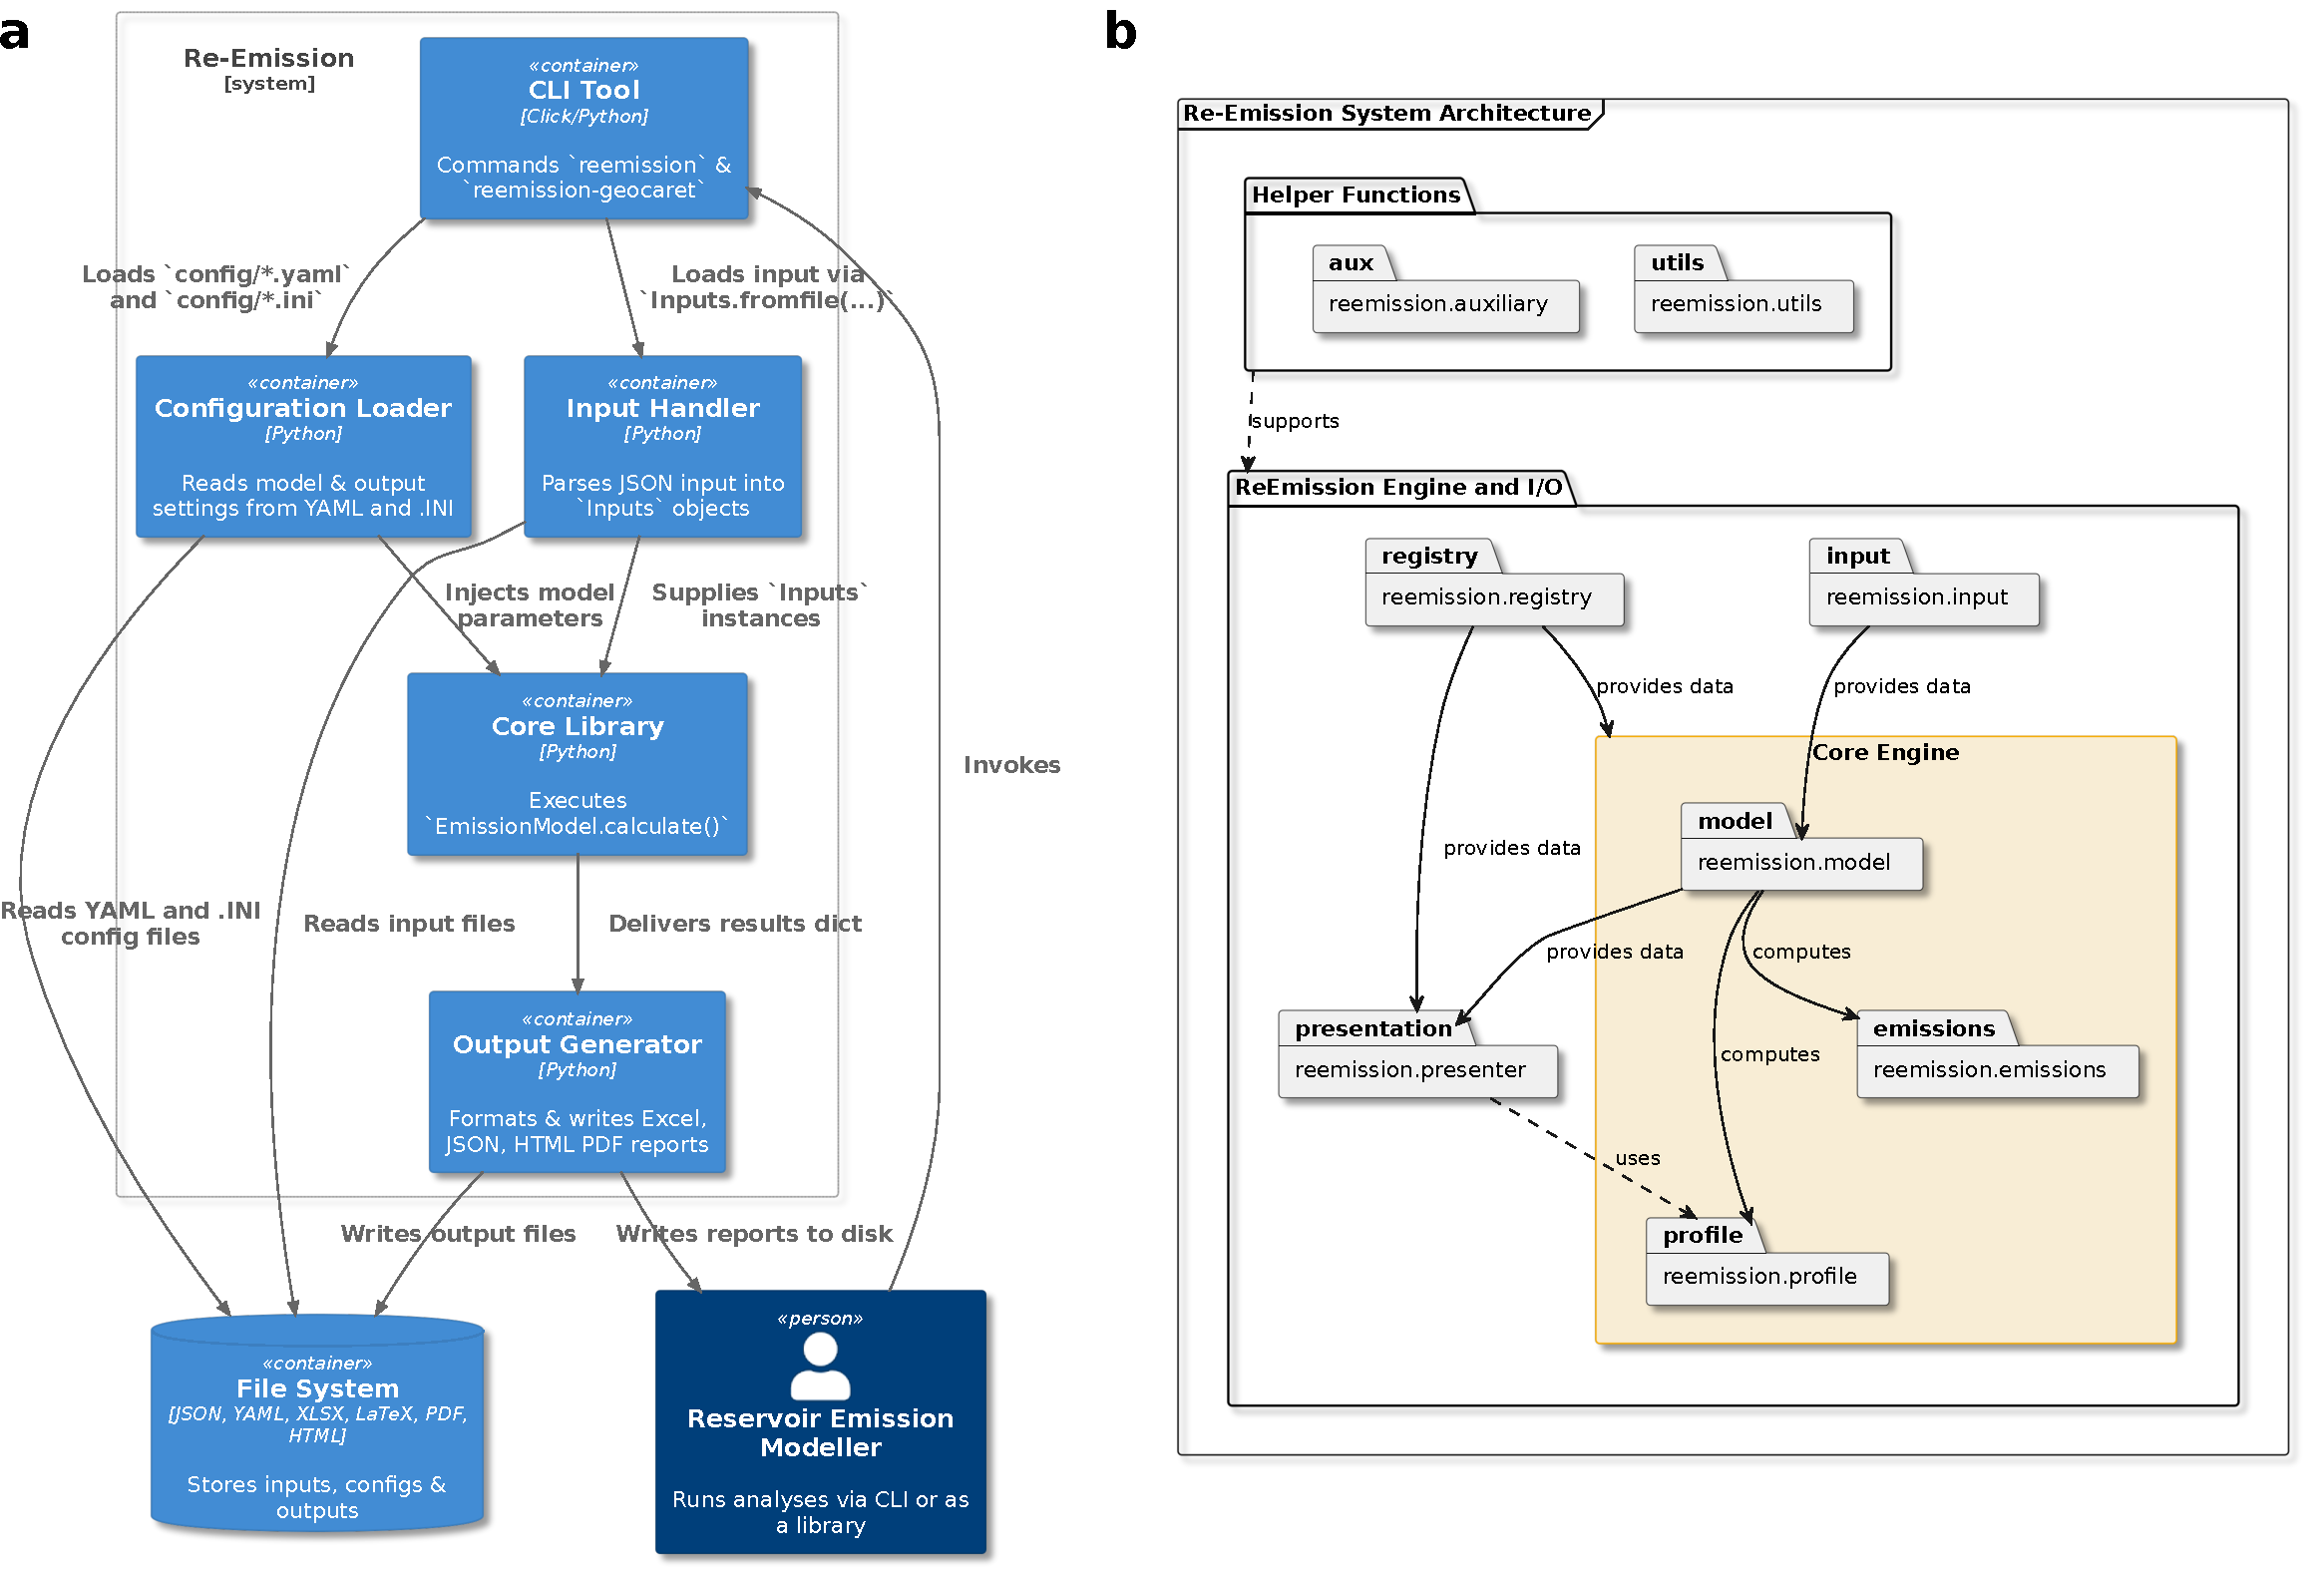
\includegraphics[width=0.99\textwidth]{figures/high_level_achitecture.pdf}
    \caption{Software architecture of the Re-Emission package. \textbf{a}, Container-level interactions showing key components, their functionalities, and data flow between system elements. Users can interact with the \acf{CLI} or Python library to orchestrate the loading of configuration parameters and input data, executes the core emission models, and generate output reports in various formats (Excel, JSON, PDF, HTML). Configuration files provide model parameters and presentation options for report and output files, while the file system stores inputs and outputs. \textbf{b}, Package dependency view illustrating the modular structure and inter-package relationships within the system architecture.}
    \label{fig:high_level_archtecture}
\end{figure}

The high-level architecture of the Re-Emission framework is illustrated in Figure~\ref{fig:high_level_archtecture}.
Re-Emission can be used either through a \acf{CLI} or by directly accessing its Core Library components from Python scripts, as shown in Figure~\figref[a]{fig:high_level_archtecture}.
The \ac{CLI} serves as the primary user interface, enabling users to perform emission analyses via simple commands.
When a command is executed, the \ac{CLI} delegates control to a configuration loader, which parses and validates the configurable model parameters, execution options (e.g., choice of submodels), and presentation settings (e.g., selection of output variables and associated metadata).
These configurations are defined in YAML and INI files located in the \vrbbrk{reemission/config/} directory and are passed to both the Core Library and \vrbbrk{reemission.presenter}; see Figure~\figref[b]{fig:high_level_archtecture}.
This design ensures a clear separation between logic (model equations) and data (model parameters and inputs).

The input data, provided in JSON format and containing reservoir, catchment, and climatic parameters, are read and parsed by \vrbbrk{reemission.input}, and converted into a strongly typed \vrbbrk{Inputs} object for use in the emission model.
This input data can be assembled either manually, by compiling information from various sources, or automatically, via an upstream reservoir and catchment processing tool such as GeoCARET~\cite{heettool}, with which Re-Emission integrates (see Section~\ref{sec:integration}).
Once the model run is completed, the results are forwarded to an output generator, where outputs are produced in several formats, including Excel workbooks (XLSX), structured JSON files, and HTML and PDF reports.
The presentation functionality is implemented in \vrbbrk{reemission.presenter}, where information about inputs, outputs, and intermediate variables is sourced from \vrbbrk{reemission.model} and \vrbbrk{reemission.profile}. 
This allows the simulation input and output information to be presented as both text and graphical visualisations.
The loading, overriding, and sharing of configuration files are managed by \vrbbrk{reemission.registry}.
%e cumulative reservoir emissions over time, based on each reservoirs' construction dates and their respective emission decay rates. 
% % -- such as regression coefficients, pre-impoundment emissions, and nutrient exports from land -- such as choice of submodels
%The input data and configuration settings are then routed into the Core Library highlighted in Figure~\figref[b]{fig:high_level_archtecture} by a lemon yellow rectangle. 
%The Core Library comprises the emission model, which runs the analysis using selected emission models and passes the results to \vrbbrk{reemission.presenter}. 

\begin{figure}[ht]
    \centering
    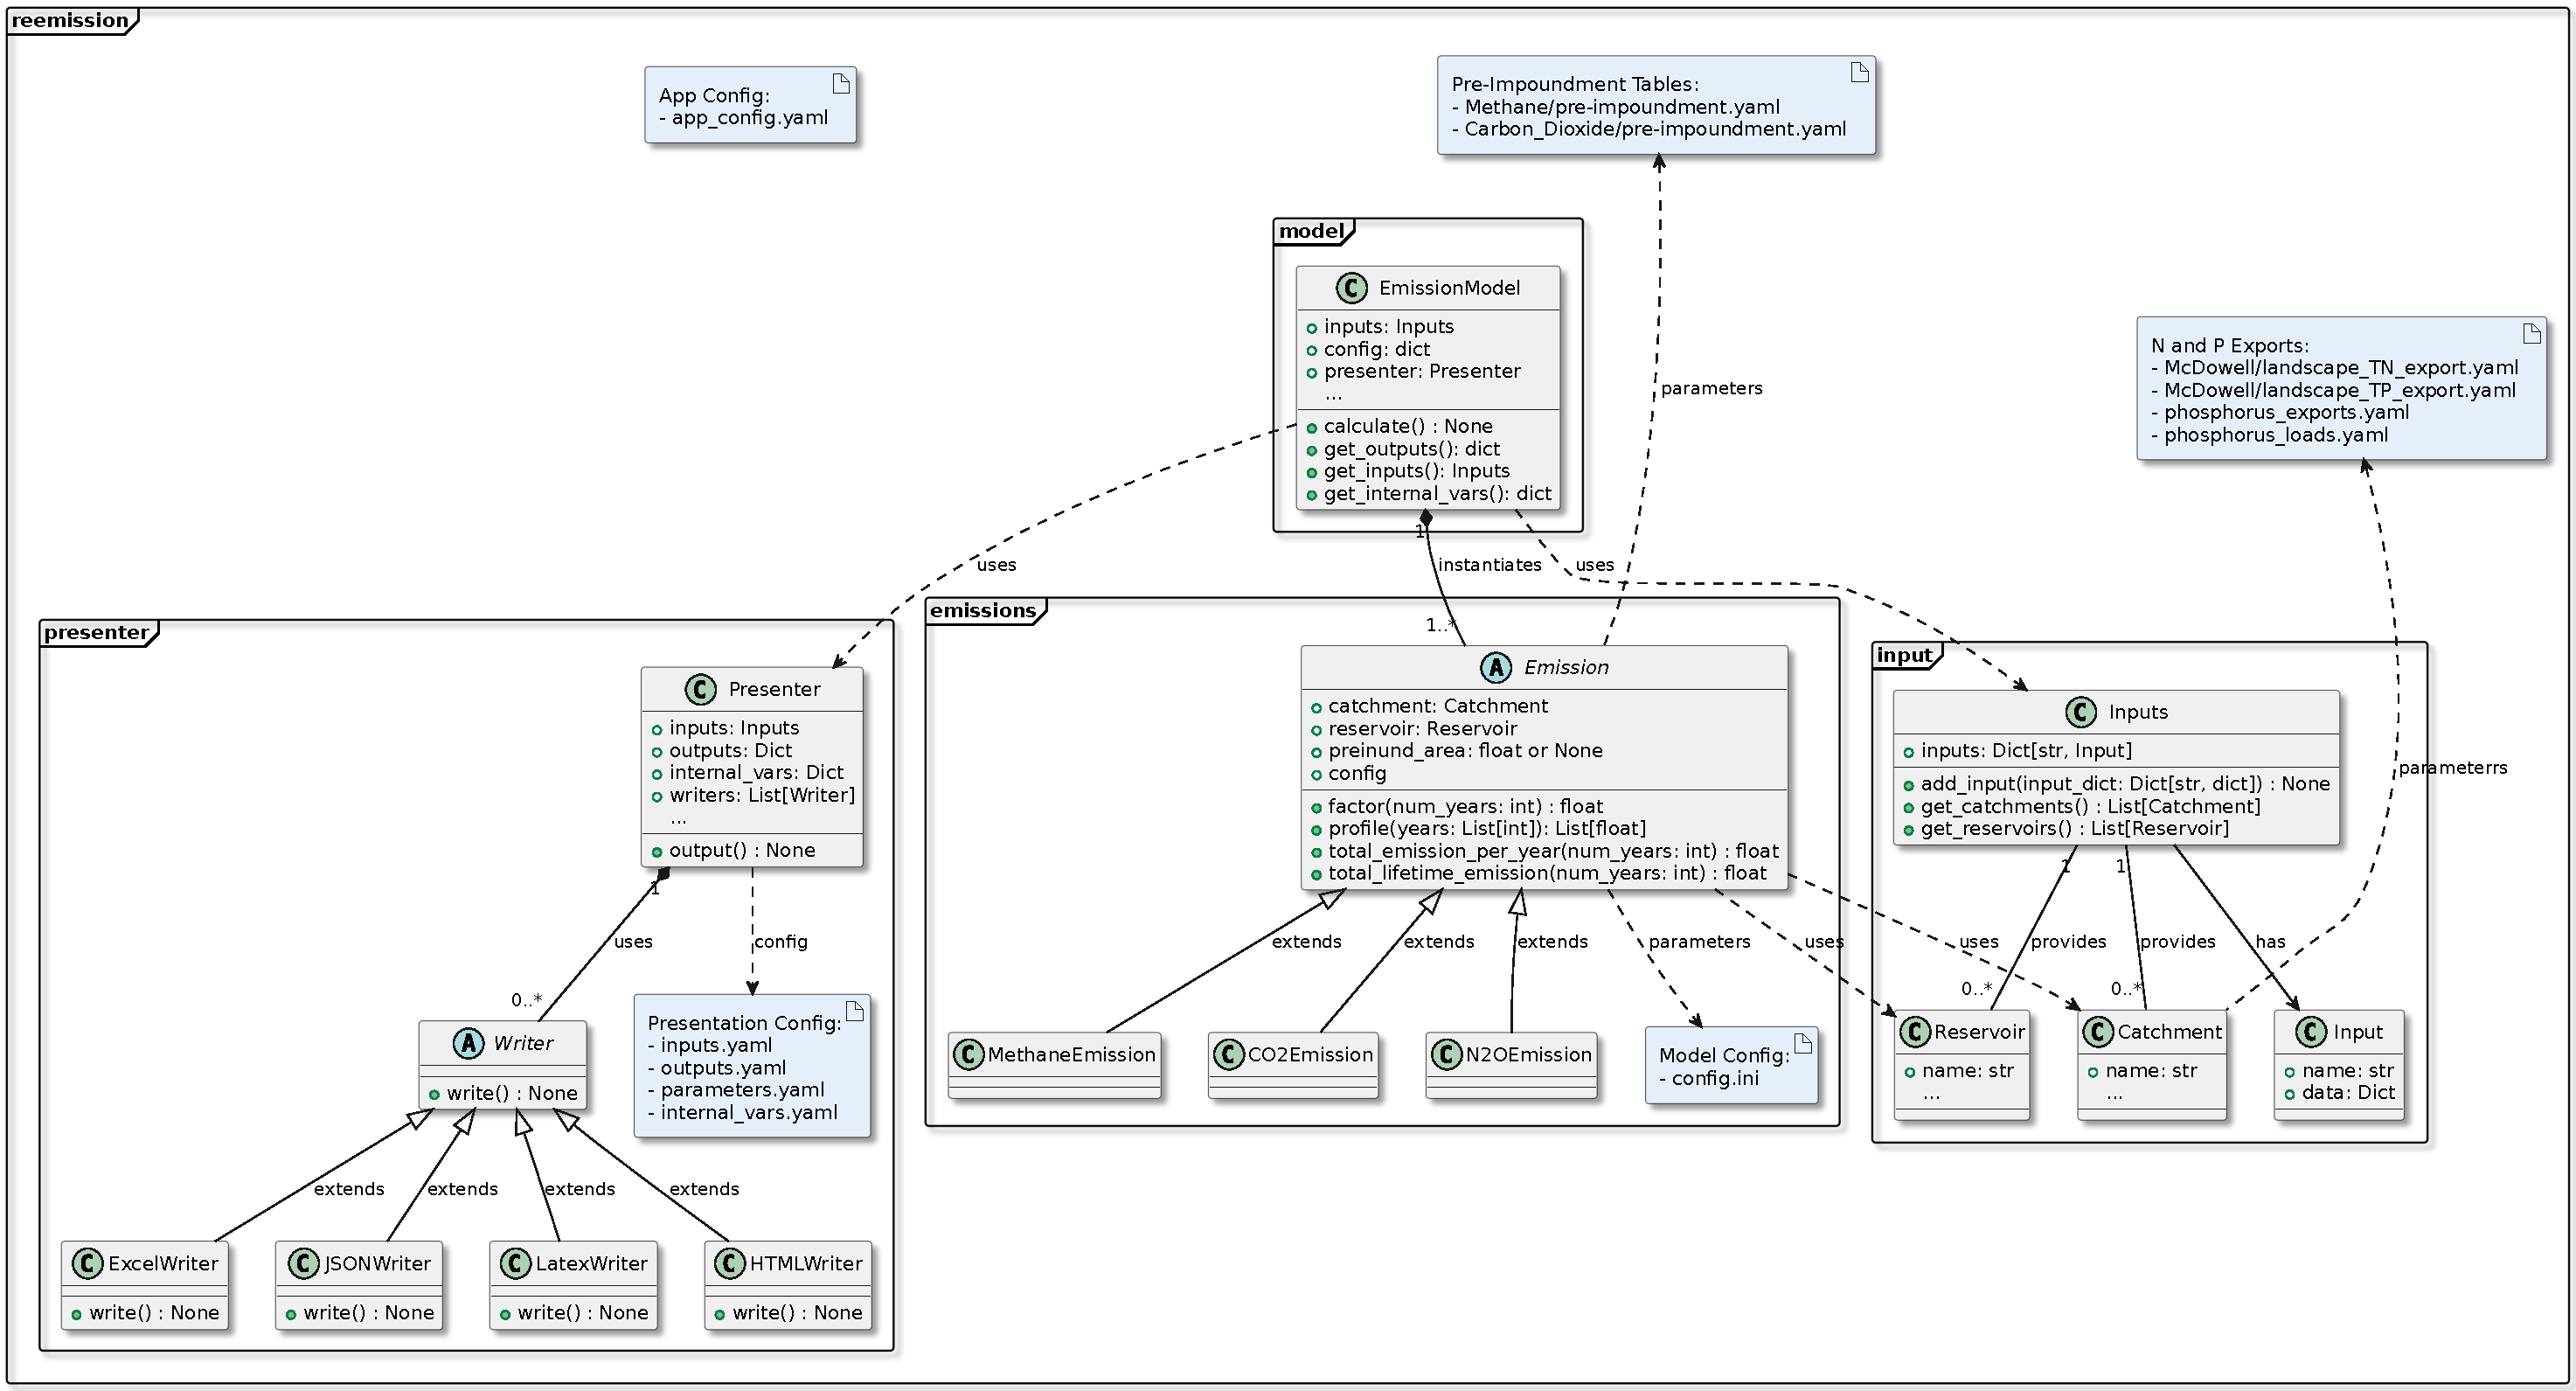
\includegraphics[width=0.99\textwidth]{figures/high_level_uml2.pdf}
	\caption{UML class diagram of the \texttt{reemission} framework, illustrating key classes and their relationships. Core components include \texttt{EmissionModel}, \texttt{Reservoir}, \texttt{Catchment}, \texttt{Emission}, \texttt{Inputs}, and \texttt{Presenter}, with abstract interfaces used to enforce modularity and extensibility.}
    \label{fig:high_level_uml}
\end{figure}

A more detailed representation of the internal structure and inter-class relationships within the modules shown in Figure~\figref[b]{fig:high_level_archtecture} is provided in the UML class diagram in Figure~\ref{fig:high_level_uml}.
The \texttt{EmissionModel} class encapsulates the simulation logic, including the instantiation of \vrbbrk{Reservoir}, \vrbbrk{Catchment}, and \vrbbrk{Emission} objects (e.g., \vrbbrk{MethaneEmission} for CH$_4$), and the subsequent calculation of \ac{GHG}-related intermediate and output variables.
The \vrbbrk{Reservoir} and \vrbbrk{Catchment} objects are supplied to \vrbbrk{EmissionModel} by the \vrbbrk{Inputs} class.
Each individual \vrbbrk{Emission} object extends the abstract \vrbbrk{Emission} class, which defines four abstract methods that must be implemented by all its subclasses.
The \vrbbrk{Presenter} class employs \vrbbrk{Writer} objects to generate outputs in various file formats. 
All \vrbbrk{Writer} objects must inherit from the abstract \vrbbrk{Writer} class, which defines a common interface for all writers.
The currently supported file formats include JSON, XLSX, PDF (via \LaTeX), and HTML.
The \vrbbrk{Reservoir}, \vrbbrk{Catchment}, \vrbbrk{Emission}, and \vrbbrk{Presenter} classes are parameterized by configuration files containing information such as regression coefficients, pre-impoundment emission factors, nutrient export rates from land, and presentation options specific to the \vrbbrk{Presenter} class.
Further details on the structure of the \vrbbrk{Reservoir} and \vrbbrk{Catchment} classes, as well as the representation of model inputs, are provided in the Appendix in Figure~\ref{fig:river_network_emissions_uml}.

\subsection{Using Re-Emission as a Python package}
\label{subsec:scripting}

Re-Emission can also be used as a library, enabling its functions and classes to be called directly within Python scripts to perform emission calculations. These calculations may be carried out step by step by manually constructing \vrbbrk{Reservoir} and \vrbbrk{Catchment} objects, followed by instantiating and executing \vrbbrk{Emission} objects, as shown in Listings~\ref{lst:em_calc_setup} and~\ref{lst:em_calc} in the Appendix. 
Alternatively, the \vrbbrk{EmissionModel} class may be used to streamline this process, as demonstrated in Listing~\ref{lst:em_calc_file}.
In addition to simplifying execution, the use of \vrbbrk{EmissionModel} enables results to be saved in multiple file formats via the \vrbbrk{Presenter} class, as shown in Listing~\ref{lst:em_calc_presentation}.

In both usage modes, the analytical workflow (excluding the presentation of results) follows an algorithmic structure illustrated in Algorithm~\ref{alg:reemission}. 
Input data and model parameters are first read from structured data and configuration files. 
The input is then validated prior to computation. Reservoir emissions are subsequently calculated for each reservoir defined in the dataset, and raw results are written to a JSON output file.

\begin{algorithm}[H]
\caption{Reservoir Emission Estimation}
\label{alg:reemission}
\SetKwInOut{Input}{Input}
\SetKwInOut{Output}{Output}

\AlgoDisplayBlockMarkers

\Input{Input file path (e.g., \texttt{input\_file.json})\\
       Configuration file path (e.g., \texttt{config\_file.yaml})}
\Output{Output file path (e.g., \texttt{output\_file.json})}

\BlankLine
Load input data from \texttt{input\_file.json}\;
\If{input is invalid}{
    Raise error and exit\;
}
Initialize model parameters from configuration file\;
\ForEach{entry in dataset}{
    Instantiate \texttt{Reservoir} and \texttt{Catchment} objects\;
    Instantiate \texttt{CarbonDioxideEmission} and \texttt{MethaneEmission} objects\;
    Estimate annual CO\textsubscript{2} and CH\textsubscript{4} fluxes and flux profiles\;
}
Save results to \texttt{output\_file.json}\;
\end{algorithm}


\subsection{Command-Line Interface}
\label{subsec:cli}

Re-Emission can also be used via a simple \acf{CLI}. 
Full usage instructions can be accessed by running \vrbbrk{reemission --help} in the terminal or console.
A typical example of a command-line invocation is shown in Listing~\ref{lst:em_calc_cli}, where input data are provided in \vrbbrk{input.json} and outputs are generated in multiple formats, including PDF, JSON, XLSX, and HTML.
In addition to performing emission calculations, the \ac{CLI} includes commands for converting and modifying input datasets. 
These are described further in Section~\ref{sec:integration}, which covers integration with upstream reservoir and catchment data processing; see also Listing~\ref{lst:integration_cli}.

\begin{minipage}{0.95\textwidth}
\begin{lstlisting}[language=bash, label={lst:em_calc_cli}, caption={Re-Emission \ac{CLI}: Emission calculations using input.json as the source of input data.}]
> reemission calculate 
    input.json
    -o output.pdf -o output.json -o output.xlsx  -o output.html
    --author "John Smith" 
    --title  "Reservoir Emissions Analysis"
\end{lstlisting}
\end{minipage}

\subsection{Input and output data format}
\label{subsec:input_output_formats}

The structure of the input and output data is illustrated in Figures~\ref{fig:input_data_format} and~\ref{fig:output_data_format}, respectively. 
The input data format is fixed and determined by the parameter requirements of the \vrbbrk{Reservoir} and \vrbbrk{Catchment} classes.
In contrast, the structure of the output data is largely configurable through YAML configuration files.
To enhance readability, only a subset of the full input and output content is shown in the figures.
In cases where data has been truncated, the omission is indicated using bold, light-blue text followed by an ellipsis (...).


\begin{figure}[ht]
    \centering
    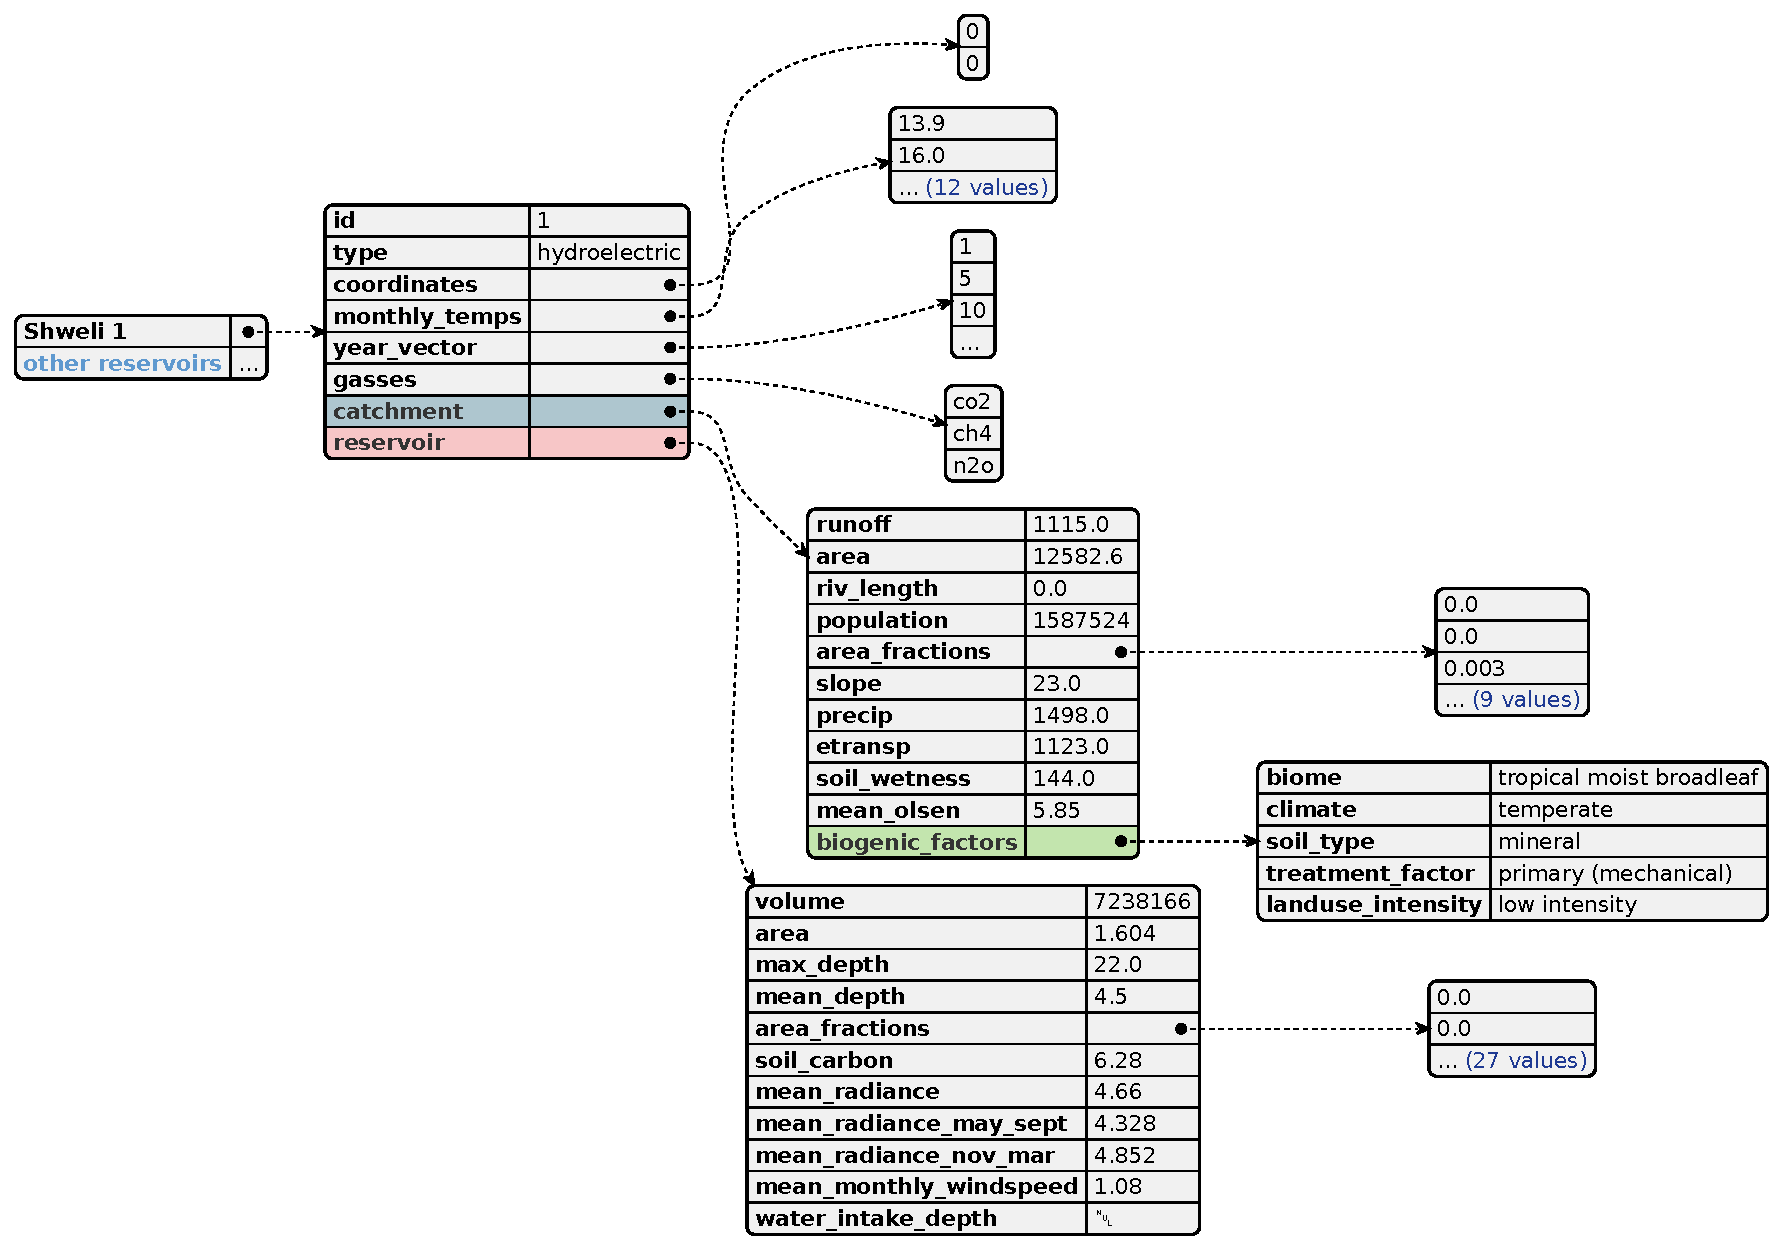
\includegraphics[width=0.75\textwidth]{figures/input_data_json.pdf}
    \caption{Structure of an input JSON file containing example data for a single reservoir. The entries related to catchment and reservoir parameters, highlighted in steel blue and salmon, correspond directly to fields in the associated \vrbbrk{Catchment} and \vrbbrk{Reservoir} class definitions, respectively. Selected values have been truncated for readability, with truncated content indicated using light blue font colour.}
    \label{fig:input_data_format}
\end{figure}

\begin{figure}[ht]
    \centering
    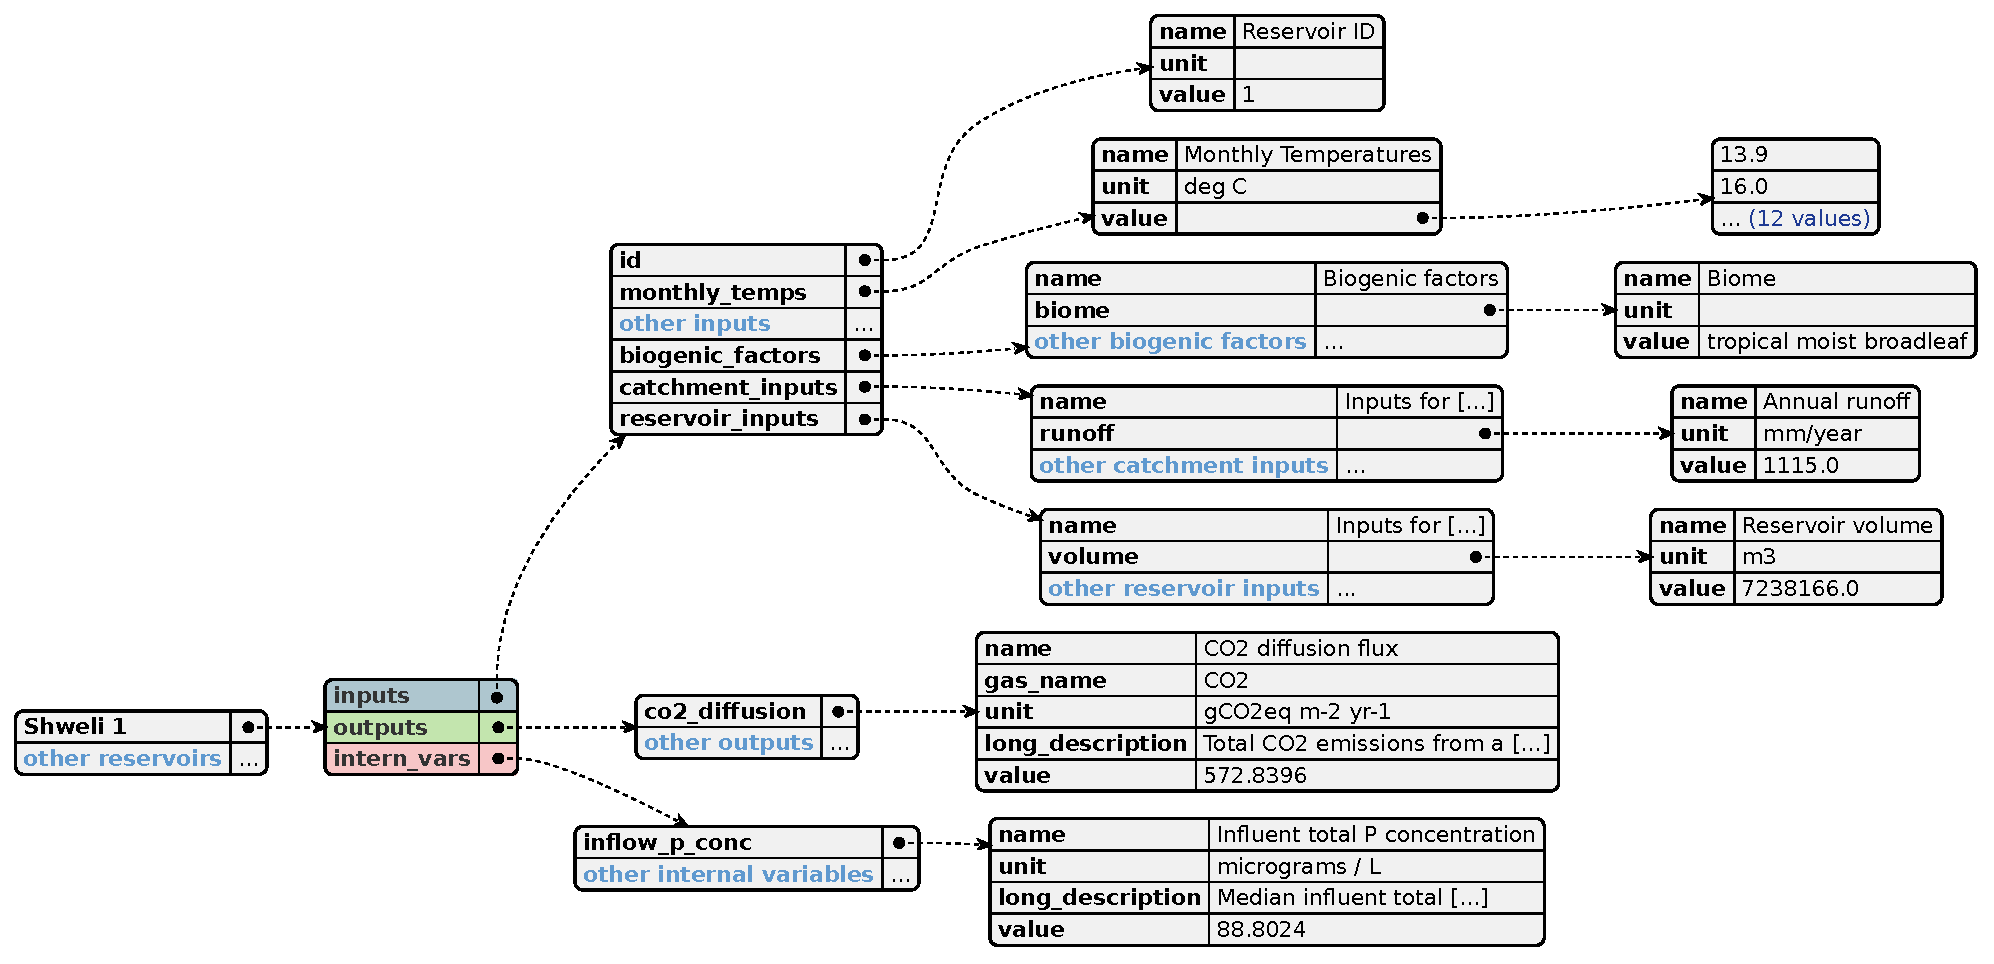
\includegraphics[width=0.9\textwidth]{figures/output_data_json.pdf}
    \caption{Structure of an example configurable output JSON file. The file is divided into three sections: inputs, outputs, and internal variables, highlighted in steel blue, olive green, and salmon, respectively. Since the number of output entries can be arbitrarily large, selected values have been truncated for readability. Truncated content is indicated using light blue font colour.}
    \label{fig:output_data_format}
\end{figure}

\subsection{Configuration options}
\label{subsec:config_options}

Configuration data -- including model parameters, options for the \vrbbrk{Presenter} class, and tabular inputs such as pre-impoundment emission factors or nutrient export coefficients -- is stored in INI and YAML files. 
These files provide semi-structured data representations that can be readily loaded into Python as dictionary objects.
The structure of these configuration files is illustrated in Figure~\ref{fig:config_uml} for presentation and model settings, Figure~\ref{fig:preimpoundment} for pre-impoundment emission factors, and Figure~\ref{fig:tp_tn_exports} for the parameterization of nutrient export models.

Configuration data is managed by the \vrbbrk{ConfigLoader} class, which registers configuration files and lazily loads them on first access. 
It also allows user-defined configurations to override default settings. 
Instances of \vrbbrk{ConfigLoader} with the registered configuration files are made globally accessible through the \vrbbrk{reemission.registry} module.

\subsection{Containerized execution using Docker}
\label{subsec:docker}

To ensure reproducibility and simplify the deployment of Re-Emission we implemented a fully containerized workflow using Docker~\cite{merkel2014docker}, GitHub Actions, and the \acf{GHCR}, as visualized in Figure~\ref{fig:docker_containerizing}. 
This approach ensures consistent runtime behaviour across systems and eliminates the need for complex setup procedures, thereby lowering the technical barriers to usage.
Docker is an open-source platform that enables packaging applications and their dependencies into standardized units called containers, which can be executed as isolated environments.
Re-Emission together with the Python interpreter, essential libraries, and other dependencies are encapsulated in a Docker image. 
The source code and Docker configuration files (\verb|compose.yaml|) are hosted in a GitHub repository, where \ac{CI} is handled via GitHub Actions.
A Docker image is automatically built and published to the GitHub Container Registry upon a push to the \verb|release| branch. 
The image can be retrieved from the web using the standard \verb|docker pull| command, provided that Docker is installed on the user's computer.

The Re-Emission \ac{CLI} is invoked using \verb|docker compose run reemission| from within a directory that contains the \verb|compose.yaml| Docker configuration file.
This file is required at runtime to map directories between the Docker container and the user's local environment, enabling access to input files and saving outputs.
To streamline the Dockerized execution of Re-Emission, we also provide a companion repository that defines the required folder structure and configuration files for running the Re-Emission container, and specifies the locations of directories for reading inputs and saving outputs~\cite{janus_geocaret_reemission}; see \emph{Software Availability}.

At present, the shared Docker images for Re-Emission do not include a \LaTeX\ distribution, which is required for generating PDF reports using the \verb|pylatex| library. 
This omission is intentional, as including a full \LaTeX\ system, such as TeX~Live, would substantially increase the size of the Docker image, making it less practical for lightweight distribution and deployment. 
As a result, PDF report generation is not currently supported in the containerized version of Re-Emission, although similar visually comparable reports can be generated in HTML format (see Section~\ref{subsec:input_output_formats}).
For users who require PDF report generation within the Docker environment, a custom Docker image must be built by extending the official Re-Emission image with a \LaTeX\ installation. 
This can be accomplished by writing a new Dockerfile (see Listing~\ref{lst:docker_with_latex}) and building the image with \verb|docker build -t reemission-with-latex .| executed in the directory containing Dockerfile.

\begin{figure}[ht]
    \centering
    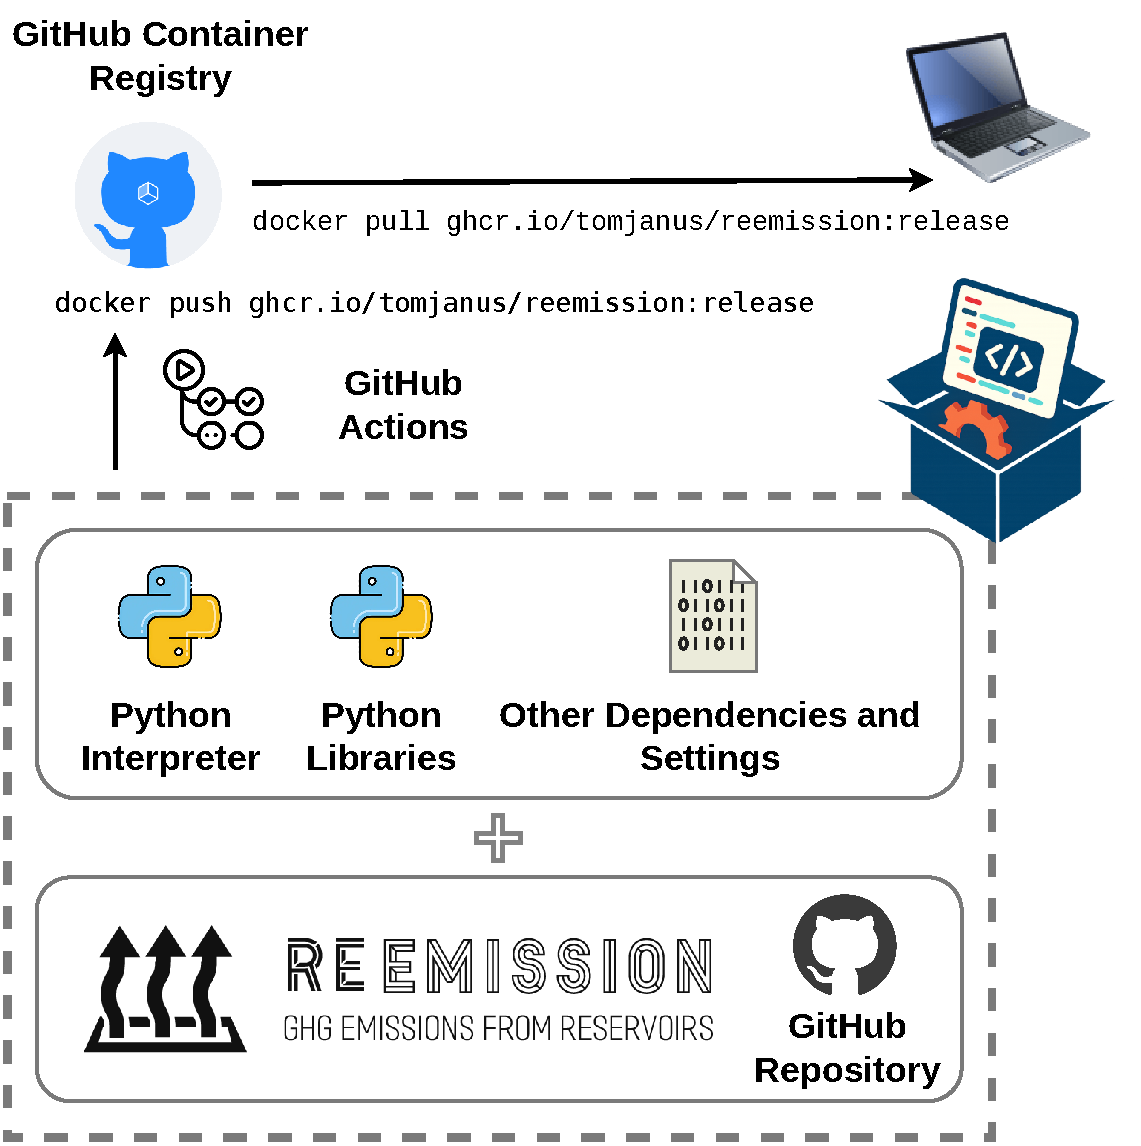
\includegraphics[width=0.55\textwidth]{figures/docker-explanation.drawio.pdf}
    \caption{{Containerized deployment of Re-Emission using Docker, GitHubActions, and the GitHub Container Registry.}}
    \label{fig:docker_containerizing}
\end{figure}

\begin{minipage}{0.95\textwidth}
\begin{lstlisting}[language=Dockerfile, , label={lst:docker_with_latex}, caption={Dockerfile for extending the Re-Emission image with a full TeX Live installation to enable PDF report generation}]
# Dockerfile
FROM ghcr.io/tomjanus/reemission:release
# Install TeX Live
RUN apt-get update && \
    apt-get install -y texlive-full && \
    apt-get clean && \
    rm -rf /var/lib/apt/lists/*
\end{lstlisting}
\end{minipage}

\section{Integration with upstream reservoir and catchment processing}
\label{sec:integration}

The principal challenge in estimating emissions from multiple reservoirs using spatially explicit emission models such as G-res lies in the manual effort and time required to source and derive the necessary input data. 
When input variables are not directly available, they must be extracted from geospatial datasets using various \ac{GIS} methods. 
This typically involves the prior delineation of each reservoir and its corresponding catchment area, followed by the processing of diverse datasets such as \acp{DEM}, land cover maps, soil and biome classification layers, and various climate-related datasets. 
These steps are often labour-intensive and time-consuming, particularly at larger spatial scales.

To streamline this process, we provide functionality for generating input JSON files for Re-Emission from the outputs of the open-source Geospatial CAtchment and REservoir analysis Tool (GeoCARET)~\cite{heettool}.
GeoCARET defines algorithms for a variety of statistical and geometric operations required to derive reservoir and catchment characteristics, and executes them on \ac{GEE}~\cite{gorelick2017google} via its Python API. 
This setup enables automated data acquisition and preprocessing across multiple reservoir sites with minimal overhead, providing the necessary inputs for the G-res model.
While GeoCARET remains in an early stage of development, it is already capable of practical application and was used to produce input data for the two case studies featured in this paper.

Integration between the tools is supported through a suite of \ac{CLI} functions, illustrated in Listing~\ref{lst:integration_cli}, that (i) merge multiple tabular files and populate missing variables (e.g., those not derivable from geospatial datasets and requiring manual input), (ii) convert tabular data to JSON format, and (iii) optionally merge individual reservoir and catchment shapefiles to facilitate the mapping and visualization of emissions. 
The integration workflow is further simplified by running both tools within their respective Docker containers, coordinated through the Re-Emission -- GeoCARET companion repository~\cite{janus_geocaret_reemission} introduced earlier; see \emph{Software Availability} for details.


\begin{minipage}{0.95\textwidth}
\begin{lstlisting}[language=bash, 
label={lst:integration_cli}, caption={Re-Emission CLI: Processing outputs from the GeoCARET reservoir and catchment processing tool.}]
# Step 1: Processing tabular GeoCARET outputs in multiple .csv files 
> reemission reemission-geocaret process-tab-outputs \
    -i  geocaret_outputs.csv \
    -o  reemission_inputs.csv \
    -cv 'c_treatment_factor' 'primary (mechanical)' \
    -cv 'c_landuse_intensity' 'low intensity' \
    -cv 'type' 'potable'
# Step 2: Creating Re-Emission input JSON file from the tabular CSV data
> reemission-geocaret tab-to-json 
    -i reemisison_inptus.csv 
    -o reemission_inputs.json
# Step 3: Merging shape files (one per individual reservoir, catchment, dam, etc.) into combined shapes per geometry type
> reemission-geocaret join-shapes \
    -i  input_folder
    -o  output_folder
    -gp 'R_*.shp, C_*.shp, PS_*.shp'
    -f  'reservoirs.shp, catchments.shp, dams.shp'
\end{lstlisting}
\end{minipage}

%% Use \subsubsection, \paragraph, \subparagraph commands to 
%% start 3rd, 4th and 5th level sections.
%% Refer following link for more details.
%% https://en.wikibooks.org/wiki/LaTeX/Document_Structure#Sectioning_commands

%% Refer following link for more details.
%% https://en.wikibooks.org/wiki/LaTeX/Floats,_Figures_and_Captions
%% https://en.wikibooks.org/wiki/LaTeX/Importing_Graphics#Importing_external_graphics

\section{Emission model validation}
\label{sec:validation}

We conducted a validation study to verify the correctness of Re-Emission’s implementation of the G-res model and to ensure that no implementation errors were introduced into the software’s core engine due to the additional complexity of the presentation, input handling, and configuration modules.

For this purpose, we independently re-implemented the G-res model based on its original formulation~\cite{Prairie2021} using the R programming language. Both implementations were used to compute final outputs (e.g., gross and net areal CO$_2$ and CH$_4$ emissions across various emission pathways) and intermediate variables involved in the emission calculations. 
By systematically comparing the outputs and inspecting the source code of both implementations, we significantly reduced the likelihood of computational discrepancies.

To evaluate model accuracy across a broad input space, we constructed a synthetic validation dataset by randomly perturbing categorical input variables.
This allowed us to explore combinations of parameter values not previously encountered in our case studies. 
The resulting dataset comprises 246 reservoirs derived from modifications to real reservoirs located in Scotland, Wales, and Myanmar. 
These inputs span a wide range of land-cover types, biomes, climate zones, soil types, land-use intensities, and catchment-wide treatment factors.

The agreement between Re-Emission and the R-based implementation of the G-res model is illustrated in Figures~\ref{fig:validation_plot_gross_emissions} and \ref{fig:validation_plot_net_emissions}. 
The results show a near-perfect match across gross areal emissions by pathway (Figure~\ref{fig:validation_plot_gross_emissions}), pre-impoundment emissions (Figure~\figref[a]{fig:validation_plot_net_emissions}), and net anthropogenic emissions (Figure~\figref[b]{fig:validation_plot_net_emissions}), with the coefficient of determination ($R^2$) equal to 1.000 in all cases.
These findings confirm that Re-Emission produces reliable estimates of reservoir emissions under a wide variety of environmental and geographical conditions.

\begin{figure}[ht]
    \centering
    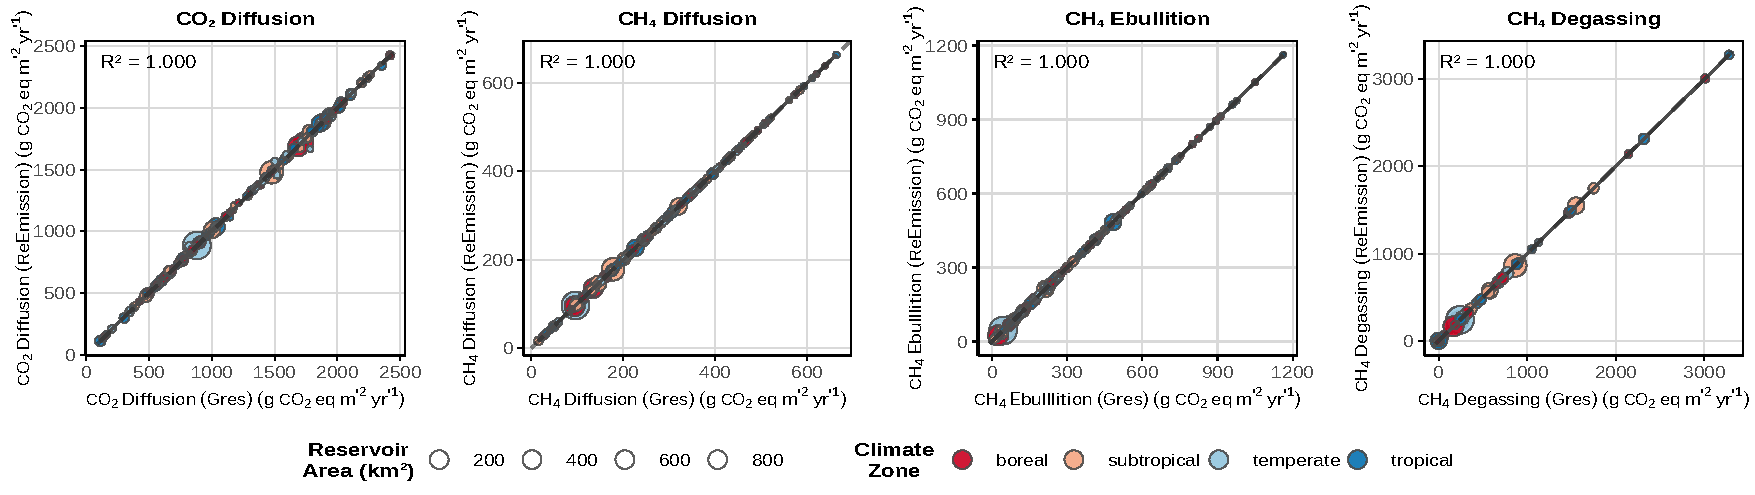
\includegraphics[width=1.0\textwidth]{figures/comparison_plot.pdf}
    \caption{{Comparison of gross areal emission rates via four emission pathways -- CO$_2$ diffusion, CH$_4$ diffusion, CH$_4$ ebullition, and CH$_4$ degassing (from left to right) -- predicted using Re-Emission (y-axis) and the R-based G-res implementation (x-axis).}}
    \label{fig:validation_plot_gross_emissions}
\end{figure}

\begin{figure}[ht]
    \centering
    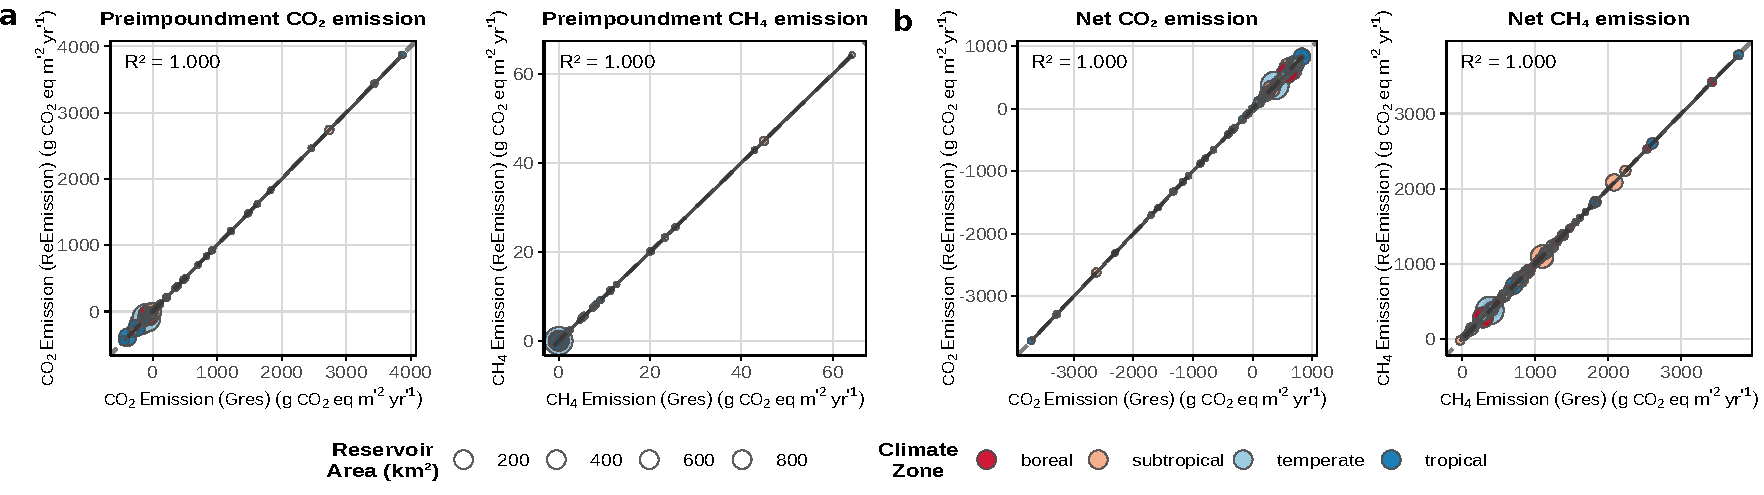
\includegraphics[width=1.0\textwidth]{figures/comparison_plot_net_emissions.pdf}
    \caption{{Comparison of (a) areal pre-impoundment CO$_2$ and CH$_4$ emissions and (b) net anthropogenic areal CO$_2$ and CH$_4$ emissions predicted using Re-Emission (y-axis) and the R-based G-res implementation (x-axis).}}
    
    \label{fig:validation_plot_net_emissions}
\end{figure}

\section{Case Studies}
\label{sec:case_studies}

We present two case studies to demonstrate the application of some of the key functionalities in Re-Emission for estimating \ac{GHG} emissions from reservoirs: (i) the estimation of total life-cycle emissions and emission profiles at scale, and (ii) the assessment of emissions under parametric uncertainty.
The first case study illustrates how Re-Emission can support emission assessments from multiple reservoirs, e.g. regionally or nationally.
The second showcases how Re-Emission can be coupled with the Python-based sensitivity analysis library SALib~\cite{Iwanaga_Toward_SALib_2_0_2022} to explore the global sensitivity and uncertainty of emission predictions in response to uncertain model parameters.
This capability is of both practical and scientific relevance: it can inform robust decision-making and contribute to advancing methodological research in reservoir emission modelling. 
To the best of our knowledge, the impact of uncertainties -- particularly input uncertainties -- on emission estimates has not received sufficient attention in the literature to date. 
Re-Emission addresses this gap by supporting uncertainty and sensitivity analyses with SALib.

\subsection{Emission trajectories from existing and planned assets in Myanmar}
\label{subsec:myanmar}

In this case study, we estimate the temporal evolution of total biogenic \ac{GHG} emissions and areal emission fluxes from more than 200 existing and planned reservoirs in Myanmar. 
Myanmar possesses substantial hydropower potential, with over 100~GW of identified capacity~\citep{EA_Myanmar}.
Although the country aims to triple its hydropower capacity by 2030~\citep{Aung2020}, the greenhouse gas implications of these proposed developments remain poorly understood. 
Moreover, biogenic emissions from existing irrigation reservoirs -- of which there are many -- have received limited attention despite their potentially significant atmospheric impact.
Using Re-Emission, we estimated emissions from all identified irrigation (IRR), multipurpose (MP), and hydropower (HP) reservoirs in Myanmar known to us. 
For each reservoir, we generated emission profiles (i.e., the temporal trajectory of biogenic emissions following impoundment) and aggregated them to derive national-scale emission trajectories.

Due to the lack of reliable construction date information for many reservoirs -- particularly existing irrigation schemes and proposed hydropower projects -- we employed a stochastic approach to scenario generation. 
Specifically, we constructed 1,000 plausible development scenarios by randomly sampling missing construction dates.
For each scenario, we simulated the temporal evolution of biogenic emissions from 1965 to 2045, thereby enabling an assessment of the timing and magnitude of peak emissions, as well as cumulative emissions over the planning horizon.
The missing construction dates for existing irrigation reservoirs were sampled from a \acf{KDE} fitted to a histogram of known construction dates.
This approach reflects historical trends in irrigation infrastructure development.
In contrast, the unknown commissioning dates for planned hydropower projects were sampled uniformly between the current year (2025) and an assumed planning horizon (2045), by which time all planned projects are assumed to become operational.

The results are presented in Figure~\ref{fig:mya_emission_profile} as ensemble plots, showing the range of possible emission trajectories, the median profile, and total emissions from irrigation reservoirs alone (IRR) as well as from all reservoirs combined (IRR + HP + MP). The results suggest that uncertainty in the construction dates of irrigation reservoirs does not substantially affect the national emission profile from irrigation assets. Emissions from these reservoirs appear to have peaked around 2005 and have been declining steadily since.
In contrast, the timing of construction for planned hydropower and multipurpose projects introduces significant uncertainty into the magnitude and timing of future emission peaks.
These projects are projected to contribute substantially to Myanmar’s biogenic \ac{GHG} emissions, with peak emissions likely to occur between 2030 and 2050.
While emissions are expected to decline sharply following the peak, they are projected to remain above current levels through at least 2060.

The insights provided by Figure~\ref{fig:mya_emission_profile} can inform national \ac{GHG} mitigation strategies and guide infrastructure planning.
With further extensions, the analytical framework demonstrated here could also incorporate other types of uncertainty -- such as model parameter uncertainty -- as described in the next case study.

\begin{figure}[ht]
    \centering
    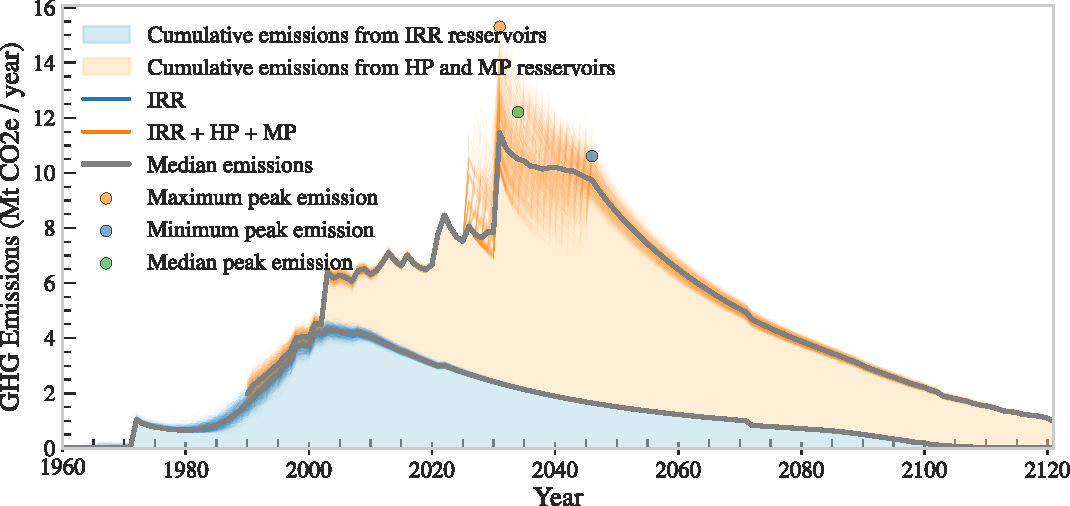
\includegraphics[width=0.8\textwidth]{figures/emission_profile.pdf}
    \caption{{Projected temporal evolution of emissions from existing and planned irrigation (IRR), multipurpose (MP), and hydroelectric (HP) reservoirs in Myanmar. In the absence of construction date information for some hydroelectric and multipurpose reservoirs, a 20-year planning horizon is assumed, by which all reservoirs included in current hydropower expansion plans are expected to be completed.}}
    \label{fig:mya_emission_profile}
\end{figure}

\subsection{Uncertainty analysis of reservoir emissions in Scotland and Wales}
\label{subsec:scotland_wales}

While it is widely acknowledged that emission model predictions are subject to considerable uncertainty, the magnitude and sources of these uncertainties remain poorly characterized. 
Reservoir emissions result from complex biogeochemical processes that are difficult to observe, model, and generalize due to their inherent spatio-temporal variability and often poorly understood dynamics.
Consequently, models developed from limited observational data may exhibit substantial epistemic and parametric uncertainties.
In addition, emission models typically rely on a large number of input variables -- many derived from geospatial datasets -- which themselves carry varying degrees of uncertainty.
These factors lead to compounded uncertainty in model outputs, with important implications for the reliability of emission estimates as a basis for decision-making and policy design.
Enabling uncertainty analysis and probabilistic emission estimation under parameter and input uncertainty is therefore of practical value to both researchers and practitioners.

Re-Emission facilitates the quantification of uncertainty arising from model parameters and inputs through an interface to the Python-based sensitivity analysis library SALib~\cite{Iwanaga_Toward_SALib_2_0_2022}.
At present, Re-Emission supports global sensitivity analysis using the Sobol method.
The interface takes advantage of Re-Emission’s flexibility to dynamically modify configuration parameters -— such as regression coefficients for emission models, pre-impoundment emission factors, or nutrient export values -- to perform both sensitivity analysis and Monte Carlo simulations under parametric uncertainty.
It also supports uncertainty quantification due to uncertain inputs.
It accommodates various probability distributions supporting continuous, discrete, and categorical variables.

To demonstrate these capabilities, we conducted an analysis of parametric uncertainty in the G-res diffusive CO$_2$ and CH$_4$ emission models and evaluated their effect on total net anthropogenic emission estimates. 
We applied this analysis to 20 reservoirs located in Wales and Scotland. 
%The results are summarized in Figure~\ref{fig:uncertainty_analysis}. 
The results show that uncertainty in total net emission estimates is largely driven by the CO$_2$ diffusion process (Figure~\figref[b]{fig:uncertainty_analysis}), particularly the ``$\textrm{k}_1\,\textrm{diff}\,\textrm{co2}$'' coefficient. Coefficients ``$\textrm{k}_6\,\textrm{diff}\,\textrm{co2}$'' and ``$\textrm{k}_1\,\textrm{diff}\,\textrm{ch4}$'' also contribute to output variability, but their influence varies across reservoirs. This suggests that their importance is context-dependent, likely influenced by site-specific conditions or the relative contribution of individual emission pathways. 
Total net emission estimates for all 20 reservoirs, along with 95\% prediction intervals, are shown in Figure~\figref[c]{fig:uncertainty_analysis}.
The variability in prediction intervals across reservoirs is evident and again largely attributable to CO$_2$ diffusion uncertainty.
Figure~\figref[d]{fig:uncertainty_analysis} presents the probability density function of total net emissions for the Baddingsgill reservoir, illustrating the spread of values and indicating the mean, median, nominal estimate, and 5$^\textrm{th}$ and 95$^\textrm{th}$ percentiles.

Although this case study is intended for demonstration purposes, the approach can be readily extended to include additional parametric and input uncertainties -- both of which are supported by Re-Emission.
Due to the computational demands of Sobol analysis, however, expanding the number of uncertain parameters may require access to high-performance parallel computing environments.
Assessing reservoir emissions under uncertainty remains an open research area, and Re-Emission provides a flexible and extensible platform for advancing such analyses.

\begin{figure}[!h]
    \centering
    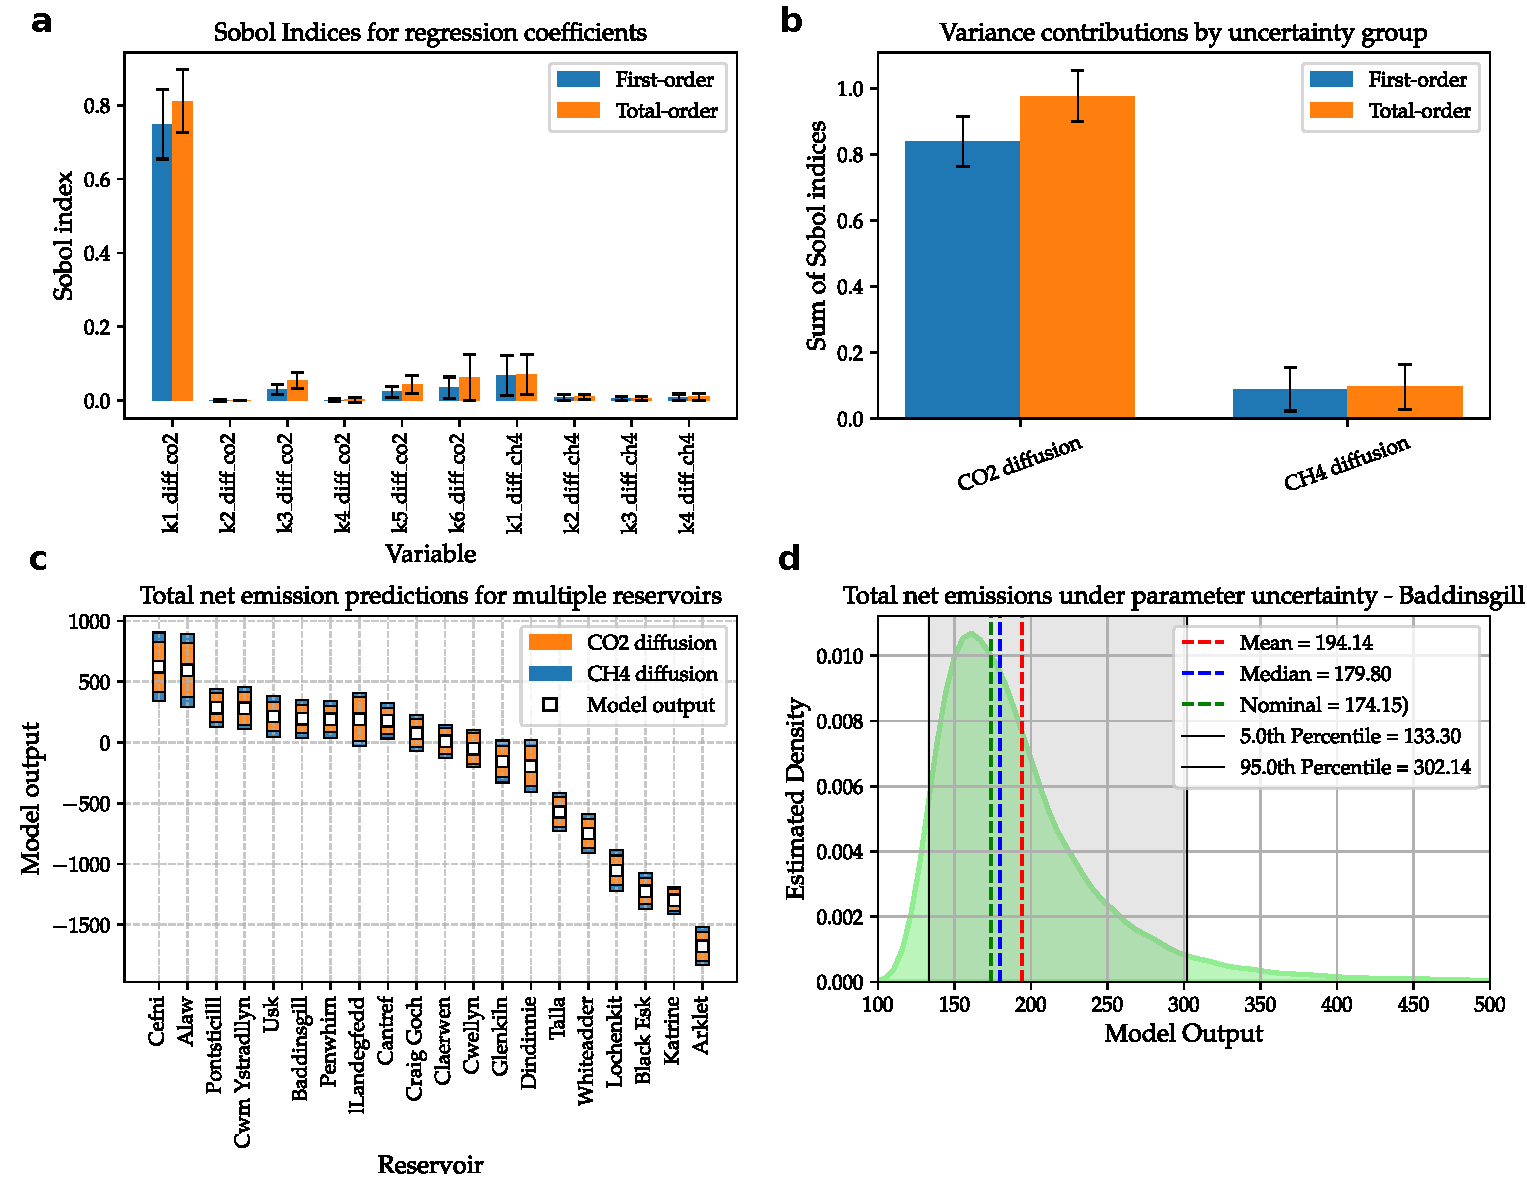
\includegraphics[width=1.0\textwidth]{figures/reemission_sobol_paper.pdf}
    \caption{
Quantification of parametric uncertainty in total net emissions from CO$_2$ and CH$_4$ diffusion processes for 20 reservoirs in Wales and Scotland. 
\textbf{(a)} First-order and total-order Sobol indices for the CO$_2$ and CH$_4$ diffusion regression coefficients, with error bars indicating variability across reservoirs. 
\textbf{(b)} Aggregated Sobol indices (first- and total-order) grouped by sources of uncertainty. 
\textbf{(c)} Total net emission estimates for the 20 reservoirs, with error bars indicating 95\% prediction intervals; the contribution of each uncertainty group is color-coded. 
\textbf{(d)} Probability density function of total net emissions for a selected reservoir, with mean, median, nominal values, and the 5$^\textrm{th}$ and 95$^\textrm{th}$ percentiles indicated.
}
    \label{fig:uncertainty_analysis}
\end{figure}


% ----- for information only ------
%The mineral/organic soil partitioning is derived from the ‘soil grids’ global layers, from which the soil C content is calculated as the mean C content of the inundated reservoir area and provided in the variable \verb|r_msocs_kgperm2|. It is required for distinguishing mineral from organic soils in the impounded/inundated reservoir area in order to apply correct \ac{IPCC} default tier1 ghg emission factors by climatezone and landcover type to estimate pre-impoundment GHG fluxes. 
%(seek definition) The organic soils are broadly peats that are positioned deeper than 40cm in the soil column and are thus somewhat restricted to specific areas (boreal, temperate uplands (Scotland), tropical uplands (andes) and basins (Congo) and SW Asia, such as Indonesia , with lots of palm on peat).
%(Chris) The general and \ac{IPCC} definition of organic soils (see image at end of this mail- I don’t find this free of ambiguity but anyway) is that they contain $>$12\% organic carbon by weight in the 0-30cm soil horizon.
%If 40 kg OC m-2 is expressed as a \% of soil volume (GRES text), with 1g OC incorrectly taken as = 1cm3 and 1cm3 soil = 1 g soil, for the 0-30cm strata, we get total mass or vol of soil in 0-30cm for 1m2 = 300kg or 300dm3 or 0.3 m3
%40 / 300 = 0.13 = 13.3\%  SOC – this is close to the threshold of 12\%   (although 36 kg m-2 would yield exactly 12\% by this approach).
%This is incorrect and indeed there are no global incidences of  $>$c.25 kg OC m-2 for the 0-30cm soil horizon. Aside from my speculation I cannot see how gres may have estimated the \% OC from the soil OC stock data (t/ha for 0-30cm), or how to consolidate their approach with the \ac{IPCC} org soil definition. 
%What we need to try to do to get correct soil classification among Min and Org soils:    derive \% SOC for 0-30cm.
% ----- for information only ------


\section{Discussion}
\label{sec:discussion}

In this manuscript, we have shown a critical gap in the current technological landscape that has hindered scientists and practitioners from estimating reservoir greenhouse gas emissions using spatially explicit models. 
To address this gap, we developed an open-source software tool that can process outputs form GeoCARET -- an automated reservoir and catchment processing framework -- to enable automated assessments of reservoir emissions.
We demonstrate the capabilities of the software through two case studies, showcasing its application in estimating emissions from large collections of reservoirs, its configurability, and its capacity for solving more advanced analyses, such as uncertainty quantification and probabilistic modelling.
While the tool offers significant improvements over existing solutions, we acknowledge several limitations that merit future development. 
These limitations, along with the tool's benefits and proposed directions for further work, are discussed in detail in the following sections.

\subsection{Limitations}
\label{subsec:limitations}

%\hl{here I would clearly partition limitations that are 'software limitations' and those that are science-data limitations}

Despite several advancements over existing software, \emph{Re-Emission} currently exhibits several limitations that merit further development.
First, the tool is currently designed primarily for implementing and extending the G-res model. 
As such, it cannot be viewed as a general-purpose framework capable of adopting diverse modelling paradigms (e.g., process-based approaches, hydrodynamic models, etc.). 
%It is limited to G-res and models that are conceptually similar.
Second, because the tool implements the G-res model along with several model extensions, it inherits the limitations, biases, and uncertainties of those models. 
While largely based on empirical dataset by \citet{Deemer2016}, comprising measurements from 167 hydropower reservoirs globally but with uneven geographical distribution, the regressions in the G-res model based on this dataset may not adequately represent the diversity of reservoir types and climatic conditions leading to biases and inaccuracies; see e.g. \citet{Hansen2022}.
%Another limitation concerns the model's reliance on significant amounts of input data that need to be derived manually from geospatial datasets for each individual reservoir; see e.g. the G-res Tool~\cite{Prairie2021}.
%This manual effort presents a substantial barrier to scaling reservoir emission assessments with G-res to larger spatial extents, such as national, regional, or global analyses.
The current implementation does not support modelling of emissions from cascading systems -- i.e., from series of reservoirs where the outflow from an upstream reservoir becomes the inflow for a downstream one. 
Finally, \emph{Re-Emission} is not yet prepared to integrate with models of emissions from other types of aquatic systems, such as rivers and streams~\cite{Rocher-Ros2023}, lakes~\cite{Zhuang2023}, or wetlands~\cite{Hu2024}. 
Although practically-relevant models for these systems are still under development, multi-system modelling will likely be essential in the future and will require tools that facilitate such model integrations. 
Advancing towards integrated assessments of catchment-scale greenhouse gas and macronutrient budgets will be crucial for developing more transparent and spatially resolved understandings of aquatic system contributions to the global carbon cycle, ultimately informing science-based reporting and decision-making.

\subsection{Benefits}
\label{subsec:benefits}

The \emph{Re-Emission} package advances the state of the art in modelling reservoir \ac{GHG} emissions by providing a programmatic solution that enables batch processing of reservoirs and facilitates the scaling of emission assessments to multiple reservoirs. 
Moreover, it systematizes the process of modelling emissions using G-res and other prospective spatially explicit models that adopt a similar conceptual framework.
Its modular architecture, combined with its open-source nature, allows users to extend the framework by incorporating new sub-models or applying custom parameterizations -- such as region-specific calibrations or updates based on new empirical data. 
he importance of such model refinements and recalibrations has recently been highlighted by \citet{Pilla2025}.
Written in Python -- one of the most widely used programming languages in the scientific and engineering communities -- the tool can be integrated easily into larger modelling frameworks. 
This opens up opportunities for a wide range of studies, including the prediction of emissions under parametric or input uncertainties and integration with other modelling frameworks -- such as the GeoCARET tool for delineating and analysing catchments and reservoirs, as demonstrated in this manuscript. 
Finally, \emph{Re-Emission} offers a free and open-source alternative to proprietary tools, enabling cost-free emission analysis for both non-commercial and commercial applications. 
Its open and automated design further enhances reproducibility and transparency in both research and applied settings.

% ----- do not use this text ------
%designed to predict gross reservoir emissions via multiple emission pathways and quantify the share of net anthropogenic emissions
% and their underlying software is still limited.
%Overall, while the science of reservoir GHGs has advanced rapidly (from isolated measurements to global models), uncertainties are still large. Key research needs include more field data from underrepresented regions and reservoir types, better monitoring of all pathways (CH4, CO2, N2O), and refinement of predictive models (e.g. incorporating remote sensing of drawdown). In parallel, practitioners benefit from emerging tools: the G-res calculator and IPCC guidelines are widely used today, and new frameworks (e.g. automated geospatial models) are being developed to integrate GHG considerations into dam planning and policy.
%current ch4 measurements from Flooded Land are not sufficiently comprehensive to support the development of accurate default emission
%factors (especially for bubbles emissions and degassing emissions). 
%there is a lack of comprehensive data on the emission rates, dominant pathways and influence of various factors on emissions in reservoirs of different sizes, morphologies and locations. 
%The work is limited by the availability of data that cover a wide range of conditions in reservoirs  and identification of processes
%The significant share of reservoir emissions in global emissions combined with a growing reservoir storage globally (27.82$\pm$0.08~km$^3$/yr observed between 1999 and 2018~\cite{Li2023}) prompts for ...
% ----- do not use this text ------

\subsection{Future Work}
\label{subsec:future_work}

To address current limitations, future development of the \emph{Re-Emission} framework will be directed towards enhancing modularity, interoperability, and flexibility to support next-generation reservoir \ac{GHG} emission assessments.
Although the current architecture is primarily centred on implementing the G-res model, we envision transitioning to a network-based architecture that represents interconnected reservoirs and river reaches. 
Such a structure would provide a more flexible foundation for modelling emissions from hydrologically connected water bodies and address limitations such as the current inability to represent cascading reservoir systems. 
In this framework, carbon and nutrient mass balances would be explicitly solved, with emissions represented as sinks and inflows from river inlets and catchment runoff as sources.
Furthermore, adopting a plugin-oriented architecture would enable flexible model configurations by supporting interchangeable emission models and alternative formulations for key sub-processes, such as the estimation of hypolimnion depth or littoral zone area. 
To enhance end-to-end automation and improve usability, tighter integration should be established with upstream geospatial analysis tools, such as GeoCARET, to streamline the automatic sourcing and processing of catchment and reservoir input data.

Beyond architectural enhancements, future work must also address underrepresented emission pathways and processes. 
Recent empirical studies have underscored the significance of previously unmodelled emission sources, such as methane emissions from sediments~\cite{gruca2011, Isidorova2019-ft} and downstream CH$_4$ degassing~\cite{Soued2022, Zhou2024}, which in some cases may constitute up to 90\% of total reservoir-related emissions~\cite{Deshmukh}. 
Accounting for these pathways will likely require coupling with complementary models or developing new modules that incorporate dynamic environmental conditions, such as water level fluctuations and wetting-drying cycles in littoral zones~\cite{Calamita2021, Ion2021} -- motivating a re-evaluation of existing modelling architectures.
Finally, although \acf{N2O} is a highly potent climate forcer, it remains the least studied of the three major \acp{GHG} in aquatic systems and is not yet routinely included in reservoir emission models. 
However, global estimates indicate that lakes and reservoirs emit substantial amounts of N$_2$O~\cite{Li2024}, and recent studies suggest that, under certain conditions—particularly in nutrient-rich or thermally stratified systems—N$_2$O emissions may rival or even exceed those of CH$_4$~\cite{Chen2025}. These findings underscore the urgent need for expanded empirical observations and for the systematic integration of \ac{N2O} emissions into reservoir modelling frameworks to more accurately represent the cumulative climatic impact of inland waters.


% ----- do not use this text ------
%A further area for exploration is the refinement of parameterizations related to nitrogen and phosphorus exports and pre-impoundment emissions, particularly for less-studied land-cover types such as wetlands or organic soils. For instance, land uses on peatlands or high-organic-content soils may exhibit distinct biogeochemical behaviour that is not currently captured in most empirical models.
%($\sim$65 Gg N$_2$O N yr$^{-1}$ in the 2010s), yet its inclusion in models remains rare. Recent studies suggest that N$_2$O emissions may rival or exceed CH$_4$ in specific contexts~\cite{Chen2025}, particularly in nutrient-rich or thermally stratified systems. These findings highlight the urgent need for additional empirical data and model integration to better represent N$_2$O dynamics within emission assessment tools.
%Collectively, these future directions will advance the \emph{Re-Emission} framework toward a comprehensive, extensible platform capable of supporting robust and policy-relevant emission modeling across scales and regions.
%To enhance end‐to‐end automation, we will improve interoperability with upstream geospatial analysis systems such as GeoCARET, enabling streamlined acquisition and formatting of catchment and reservoir input data. A common interface layer will be defined to standardize model input specifications, perform rigorous input validation, and manage metadata across diverse model components. This interface will facilitate the substitution of custom or third‐party data sources while ensuring consistency in variable naming, units, and quality control. Collectively, these enhancements will yield a more extensible, modular platform capable of supporting complex reservoir networks and diverse emission‐modeling strategies in large‐scale assessments.
%Recently, empirical studies addressed previously not researched emission mechanisms such as methane emissions from sediments~\cite{gruca2011, Isidorova2019-ft} and downstream CH$_4$ emissions~\cite{Soued2022} -- albeit the empirical models have not been formulated.
%larger groups of reservoirs for e.g. policy-making, country-wide emission assessments or integrating within larger planning studies, such as water, energy, food, etc.
%Experiment with parameterizations such as N and P exports and pre-impoundment emissions for less explored land-cover types, e.g. land uses on organic soils - \hl{give examples}
%Recent findings show that emission processes extend beyond reservoirs and can include downstream methane degassing~\cite{Zhou2024}, carbon peaking phenomena~\cite{Calamita2021}, and alterations in nutrient and organic matter fluxes that influence microbial processes and greenhouse gas production~\cite{Ion2021}. 
%In some cases, downstream emissions may account for up to 90\% of total reservoir-related emissions~\cite{Deshmukh}.
%Accurate modelling of these processes may require coupling with multiple complementary models or the adoption of more comprehensive frameworks that capture dynamic effects such as emissions driven by water level fluctuations or wetting-drying cycles in littoral zones.
%Unmeasured pathways are also a concern: as discussed above, drawdown-zone fluxes (CO2-dominated) were omitted in most studies, and nitrous oxide (N2O) -- a potent GHG -- has been sparsely measured. Recent analyses highlight that reservoirs and lakes are significant N2O emitters (globally ∼65 Gg N2O-N·yr-1 from lakes/reservoirs in 2010s
%From within three dominant gasses, N$_2$O emissions are least researched but may be significant under specific conditions, warranting further research, which results should be integrated into models and tools. 
%Modeling for Chinese dams suggests N2O may soon surpass CH4 in some contexts \cite{Chen2025}, underscoring a new knowledge need.  
% IPCC highlight considerable data gaps with respect to CH$_4$ emissions -- for example lack of emission data for major reservoir-bearing countries such as India, China and Russia. 
% ----- do not use this text ------

\section{Conclusions}
\label{sec:conclusions}

The \emph{Re-Emission} package constitutes a significant advancement toward the standardized, transparent, and reproducible estimation of \acl{GHG} emissions from reservoirs. 
By implementing the state-of-the-art G-Res model within an open-source Python environment, it provides researchers and practitioners with a flexible platform to apply, extend, and experiment with reservoir emission modelling across diverse contexts.
Through integration with GeoCARET, the package further enables automated emission estimation with minimal manual input, facilitating automated analyses of multiple reservoirs, as demonstrated in the two case studies presented. 
Despite current limitations and ongoing development needs, \emph{Re-Emission} is already suitable for practical applications, including the assessment of emissions from individual reservoirs, regional and national reservoir infrastructure evaluations, and integration into more complex analyses such as strategic planning in the \ac{WEFE} nexus.
Importantly, the development of this tool aligns with the recommendations of the \emph{2019 Refinement to the 2006 \acs{IPCC} Guidelines for National Greenhouse Gas Inventories: Wetlands}~\cite{IPCC2019}, which advocate for the use of Tier~2 or Tier~3 methodologies, such as G-Res, to reduce uncertainty in emissions estimates where sufficient data and analytical resources become available.

%Building on the foundations of the G-res model, this study proposes an enhanced approach that requires minimal input data. By using only the location and height of a proposed hydropower dam, a suite of hydro-morphological parameters describing the catchment and reservoir can be derived. These parameters are then employed to estimate \ac{GHG} emission trajectories over a 100-year period, leveraging empirical relationships between physical characteristics and emission rates. This approach enables rapid, spatially explicit assessments of potential reservoir emissions and supports strategic planning in dam development and climate impact mitigation.

%- The paper emphasizes the need for integrated modelling approaches that combine empirical data with mechanistic understanding to improve the accuracy of \ac{GHG} emission estimates~\citet{Zhao2021}  
%Despite of over two decades of research, 
%The community would benefit from having an open-source tool for experimenting with new models, model refinement, calibration to new data, etc.

% ------------------------
%While such methods allow estimating emissions from multiple reservoirs with minimal overhead, they were found to introduce significant biases and inaccuracies, especially for reservoirs with unique properties that fell outside the range of observed data~\cite{Harrison2021}. 
%located only in specific regions in the world and of certain morphological characteristics that are not representative of 
%In place of directly calculated values, recent studies on global reservoir emission assessments~\cite{Barros2011, Deemer2016, Harrison2021, Soued2022} and reservoir investment planning~\cite{Almeida2019, Flecker2022, Carlino2024} . 
%Yet there are limited studies \citep{Almeida2019, Soued2022} that detail emissions from future dams which is based on averaged emission rates per unit of surface area that rely on limited number of empirical studies.
%Apply these emission factors to assess emissions from future reservoirs~\cite{Almeida2019, Flecker2022, Tangi2024, Carlino2024}
%Reliable estimation of reservoir emissions is essential for understanding their current and potential future impacts on the global climate, and requires accurate models and scalable tools capable of assessing emissions across large ensembles of reservoirs.

\section{Software availability}
\label{sec:software_availability}
This paper describes the software in its current state of development, including all UML diagrams, code listings, and results. All such materials correspond to specific versions of the source code: commit \texttt{93944bd} for Re-Emission and commit \texttt{30a0796} for the Re-Emission–GeoCARET integration (see detailed information about both packages below).
The manuscript source files in \LaTeX, including all figures, as well as the Python and R scripts used to generate the case study results and validation plots, are available at \href{https://github.com/tomjanus/reemission-paper}{https://github.com/tomjanus/reemission-paper}.
In addition, the repository, along with all intermediate and final outputs, is archived on Zenodo at \href{https://doi.org/10.5281/zenodo.16424011}{doi:10.5281/zenodo.16424011}.

\begin{description}
  \item[\textbf{Name of the software:}] \texttt{Re-Emission}
  \item[\textbf{Developers:}] Tomasz Janus
  \item[\textbf{Contact address:}] \href{mailto:tomasz.janus@manchester.ac.uk}{tomasz.janus@manchester.ac.uk}, \href{mailto:tomasz.k.janus@gmail.com}{tomasz.k.janus@gmail.com}
  \item[\textbf{Year first available:}] 2022
  \item[\textbf{Hardware required:}] Windows 7, 10 (tested), 11, Linux (tested on Ubuntu 22.04), MacOSX
  \item[\textbf{Software required:}] \LaTeX \, (optional)
  \item[\textbf{Program language:}] Python 3.10+
  \item[\textbf{License:}] GNU General Public Licence v3
  \item[\textbf{Availability and cost:}] free and open source
  \item[\textbf{Source code:}] \href{https://github.com/tomjanus/reemission}{https://github.com/tomjanus/reemission} %and \href{https://pypi.org/project/pyclmuapp}{PyPI}
  \item[\textbf{Package:}] \href{https://github.com/tomjanus/reemission/pkgs/container/reemission}{https://github.com/tomjanus/reemission/pkgs/container/reemission}
  %\item[\textbf{Distribution:}] \hl{Put on PyPi and maybe also on conda-forge if straightforward to do - in case we do both, add two entries: Distribution (PyPi) and Distribution (conda-forge)}
  \item[\textbf{Documentation:}] \href{https://tomjanus.github.io/reemission}{https://tomjanus.github.io/reemission}
\end{description}

\vspace{3pt}

\begin{description}
  \item[\textbf{Name of the software:}] \texttt{Re-Emission GeoCARET Integration}
  \item[\textbf{Developers:}] Tomasz Janus
  \item[\textbf{Contact address:}] \href{mailto:tomasz.janus@manchester.ac.uk}{tomasz.janus@manchester.ac.uk}, \href{mailto:tomasz.k.janus@gmail.com}{tomasz.k.janus@gmail.com}
  \item[\textbf{Year first available:}] 2024
  \item[\textbf{Hardware required:}] Platform-independent
  \item[\textbf{Software required:}] Docker, \LaTeX \, (optional)
  \item[\textbf{Program language:}] YAML configuration
  \item[\textbf{License:}] GNU General Public Licence v3
  \item[\textbf{Availability and cost:}] free and open source, requires Google Earth Engine and Google Cloud registrations
  \item[\textbf{Source code:}] \href{https://github.com/tomjanus/geocaret-reemission}{https://github.com/tomjanus/geocaret-reemission}
  \item[\textbf{Packages:}] \href{https://github.com/tomjanus/reemission/pkgs/container/reemission}{https://github.com/tomjanus/reemission/pkgs/container/reemission}
\end{description}

\section{Declaration of competing interest}
The authors declare that they have no known competing financial interests or personal relationships that could have appeared to influence the work reported in this paper.

\section{Acknowledgements}
The authors would like to acknowledge the assistance provided by the Research IT Group at the University of Manchester, in particular James Sinnott, for their help in containerizing our software using Docker.
The development of the methodology and of the early version of Re-Emission and the Myanmar case study was supported by the UK Economic and Social Research Council's Global Challenges Research Fund (GCRF) as part of the UK Research and Innovation (UKRI) Funded FutureDAMS project(\href{www.futuredams.org}{ES/P011373/1}).
Work on containerising Re-Emission and Re-Emission GeoCARET integration was partially funded by UoM's Open Research Accelerator fund.
The case study on emission uncertainty quantification for UK reservoirs was funded by UoM's Policy@Manchester fund.
Further funding for T.J., J.K.and X.Z. was provided by their institutions. 
The work of C.B. was supported by the UK Centre for Ecology and Hydrology (UKCEH). 
Any opinions, findings, and conclusions or recommendations expressed in this material are those of the authors but not necessarily the funders.

%% The Appendices part is started with the command \appendix;
%% appendix sections are then done as normal sections
\appendix

\section{Selected Code Listings}
\label{app1}

\begin{minipage}{\textwidth}
\begin{lstlisting}[language=PythonReemission, label={lst:em_calc_setup}, caption={Use of Re-Emission as a library: step-by-step problem formulation.}]
from reemission.temperature import MonthlyTemperature
from reemission.emissions   import CarbonDioxideEmission, NitrousOxideEmission, MethaneEmission
from reemission.constants   import Landuse, Climate, SoilType, Biome, TreatmentFactor, LanduseIntensity
from reemission.catchment   import Catchment
from reemission.reservoir   import Reservoir
from reemission.biogenic    import BiogenicFactors

mt = MonthlyTemperature(
  [10.56,11.99,15.46,18.29,20.79,22.09,
   22.46,22.66,21.93,19.33,15.03,11.66])
coordinates = [22.6, 94.7] # Latitude and Longitude
biogenic_factors    = BiogenicFactors(
  biome             = Biome.TROPICALMOISTBROADLEAF,
  climate           = Climate.TROPICAL,
  soil_type         = SoilType.MINERAL,
  treatment_factor  = TreatmentFactor.NONE,
  landuse_intensity = LanduseIntensity.LOW)
catchment_area_fractions = \
  [0.0, 0.0, 0.0, 0.0, 0.0, 0.01092, 0.11996, 0.867257, 0.0]
reservoir_area_fractions = [
  0.0, 0.0, 0.0, 0.0, 0.0, 0.45, 0.15, 0.4, 0.0, 
  0.0, 0.0, 0.0, 0.0, 0.0, 0.0,  0.0,  0.0, 0.0, 
  0.0, 0.0, 0.0, 0.0, 0.0, 0.0,  0.0,  0.0, 0.0]
catchment_inputs = {
  'runoff'     : 1685.6, 'area'         : 78203, 'population' : 8463, 
  'riv_length' : 9.2,    'slope'        : 8.0,   'precip'     : 2000,   
  'etransp'    : 400,    'soil_wetness' : 140,   'mean_olsen' : 5.85, 
  'biogenic_factors' : biogenic_factors,
  'area_fractions'   : catchment_area_fractions}
reservoir_inputs = {
  'volume'       : 7.66E6, 'area': 100.6,       'max_depth'         : 32.0, 
  'mean_depth'   : 13.6,   'soil_carbon': 10.2, 'water_intake_depth': 20.0
  'mean_radiance': 4.5,    
  'mean_monthly_windspeed': 3.8, 'mean_radiance_may_sept': 4.5, 
  'mean_radiance_nov_mar' : 3.2, 'area_fractions': reservoir_area_fractions
}    
year_profile = (1, 5, 10, 20, 30, 40, 50, 65, 80, 100)
catchment = Catchment(**catchment_inputs)
reservoir = Reservoir(
  **reservoir_inputs,        temperature = mt,
  coordinates = coordinates, inflow_rate = catchment_1.discharge)
\end{lstlisting}
\end{minipage}

\begin{minipage}{\linewidth}
\begin{lstlisting}[language=PythonReemission, label={lst:em_calc}, caption={Use of Re-Emission as a library: calculation of CO$_2$ and CH$_4$ emissions using \texttt{CarbonDioxideEmission} and \texttt{MethaneEmission} classes.}]
em_co2 = CarbonDioxideEmission(
  catchment = catchment_1,            reservoir     = reservoir_1,
  eff_temp  = mt.eff_temp(gas='co2'), p_calc_method = 'g-res')
co2_emission_profile = em_co2.profile(years = year_profile)
co2_emission_factor  = em_co2.factor()    # Gross emission flux
co2_net_total        = em_co2.net_total() # Net anthropogenic emission flux
em_ch4 = MethaneEmission(
	catchment = catchment_1, reservoir = reservoir_1, monthly_temp = mt)
ch4_ebullition       = em_ch4.ebullition_flux_int() # Gross ebullition flux
ch4_emission_factor  = em_ch4.diffusion_flux_int()  # Gross diffusion flux
ch4_degassing_flux   = em_ch4.degassing_flux_int()  # Gross degassing flux
\end{lstlisting}
\end{minipage}

\begin{minipage}{\linewidth}
\begin{lstlisting}[language=PythonReemission, label={lst:em_calc_file}, caption={Use of Re-Emission as a library: calculation of reservoir emissions with inputs read from file using the \texttt{Input} class.}]
from reemission.input import Inputs
from reemission.model import EmissionModel
from reemission.utils import get_package_file
input_data    = Inputs.fromfile('inputs.json')
output_config = get_package_file('config', 'outputs.yaml').as_posix()
model         = EmissionModel(
  inputs  = input_data, 
  config  = output_config, 
  p_model = 'g-res'
)
model.calculate()
print(model.outputs)
\end{lstlisting}
\end{minipage}

\begin{minipage}{\linewidth}
\begin{lstlisting}[language=PythonReemission, label={lst:em_calc_presentation}, caption={Use of Re-Emission as a library: saving results in multiple file formats using the \texttt{Presenter} and \texttt{Writer} classes.}]
from reemission.presenter import JSONWriter, LatexWriter, HTMLWriter
model.add_presenter(
  writers=[JSONWriter, LatexWriter, HTMLWriter, ExcelWriter],
  output_files=['output.json', 'output.pdf', 'output.html', 'output.xlsx'])
model.calculate()
model.save_results()
\end{lstlisting}
\end{minipage}

\begin{figure}[ht]
    \centering
    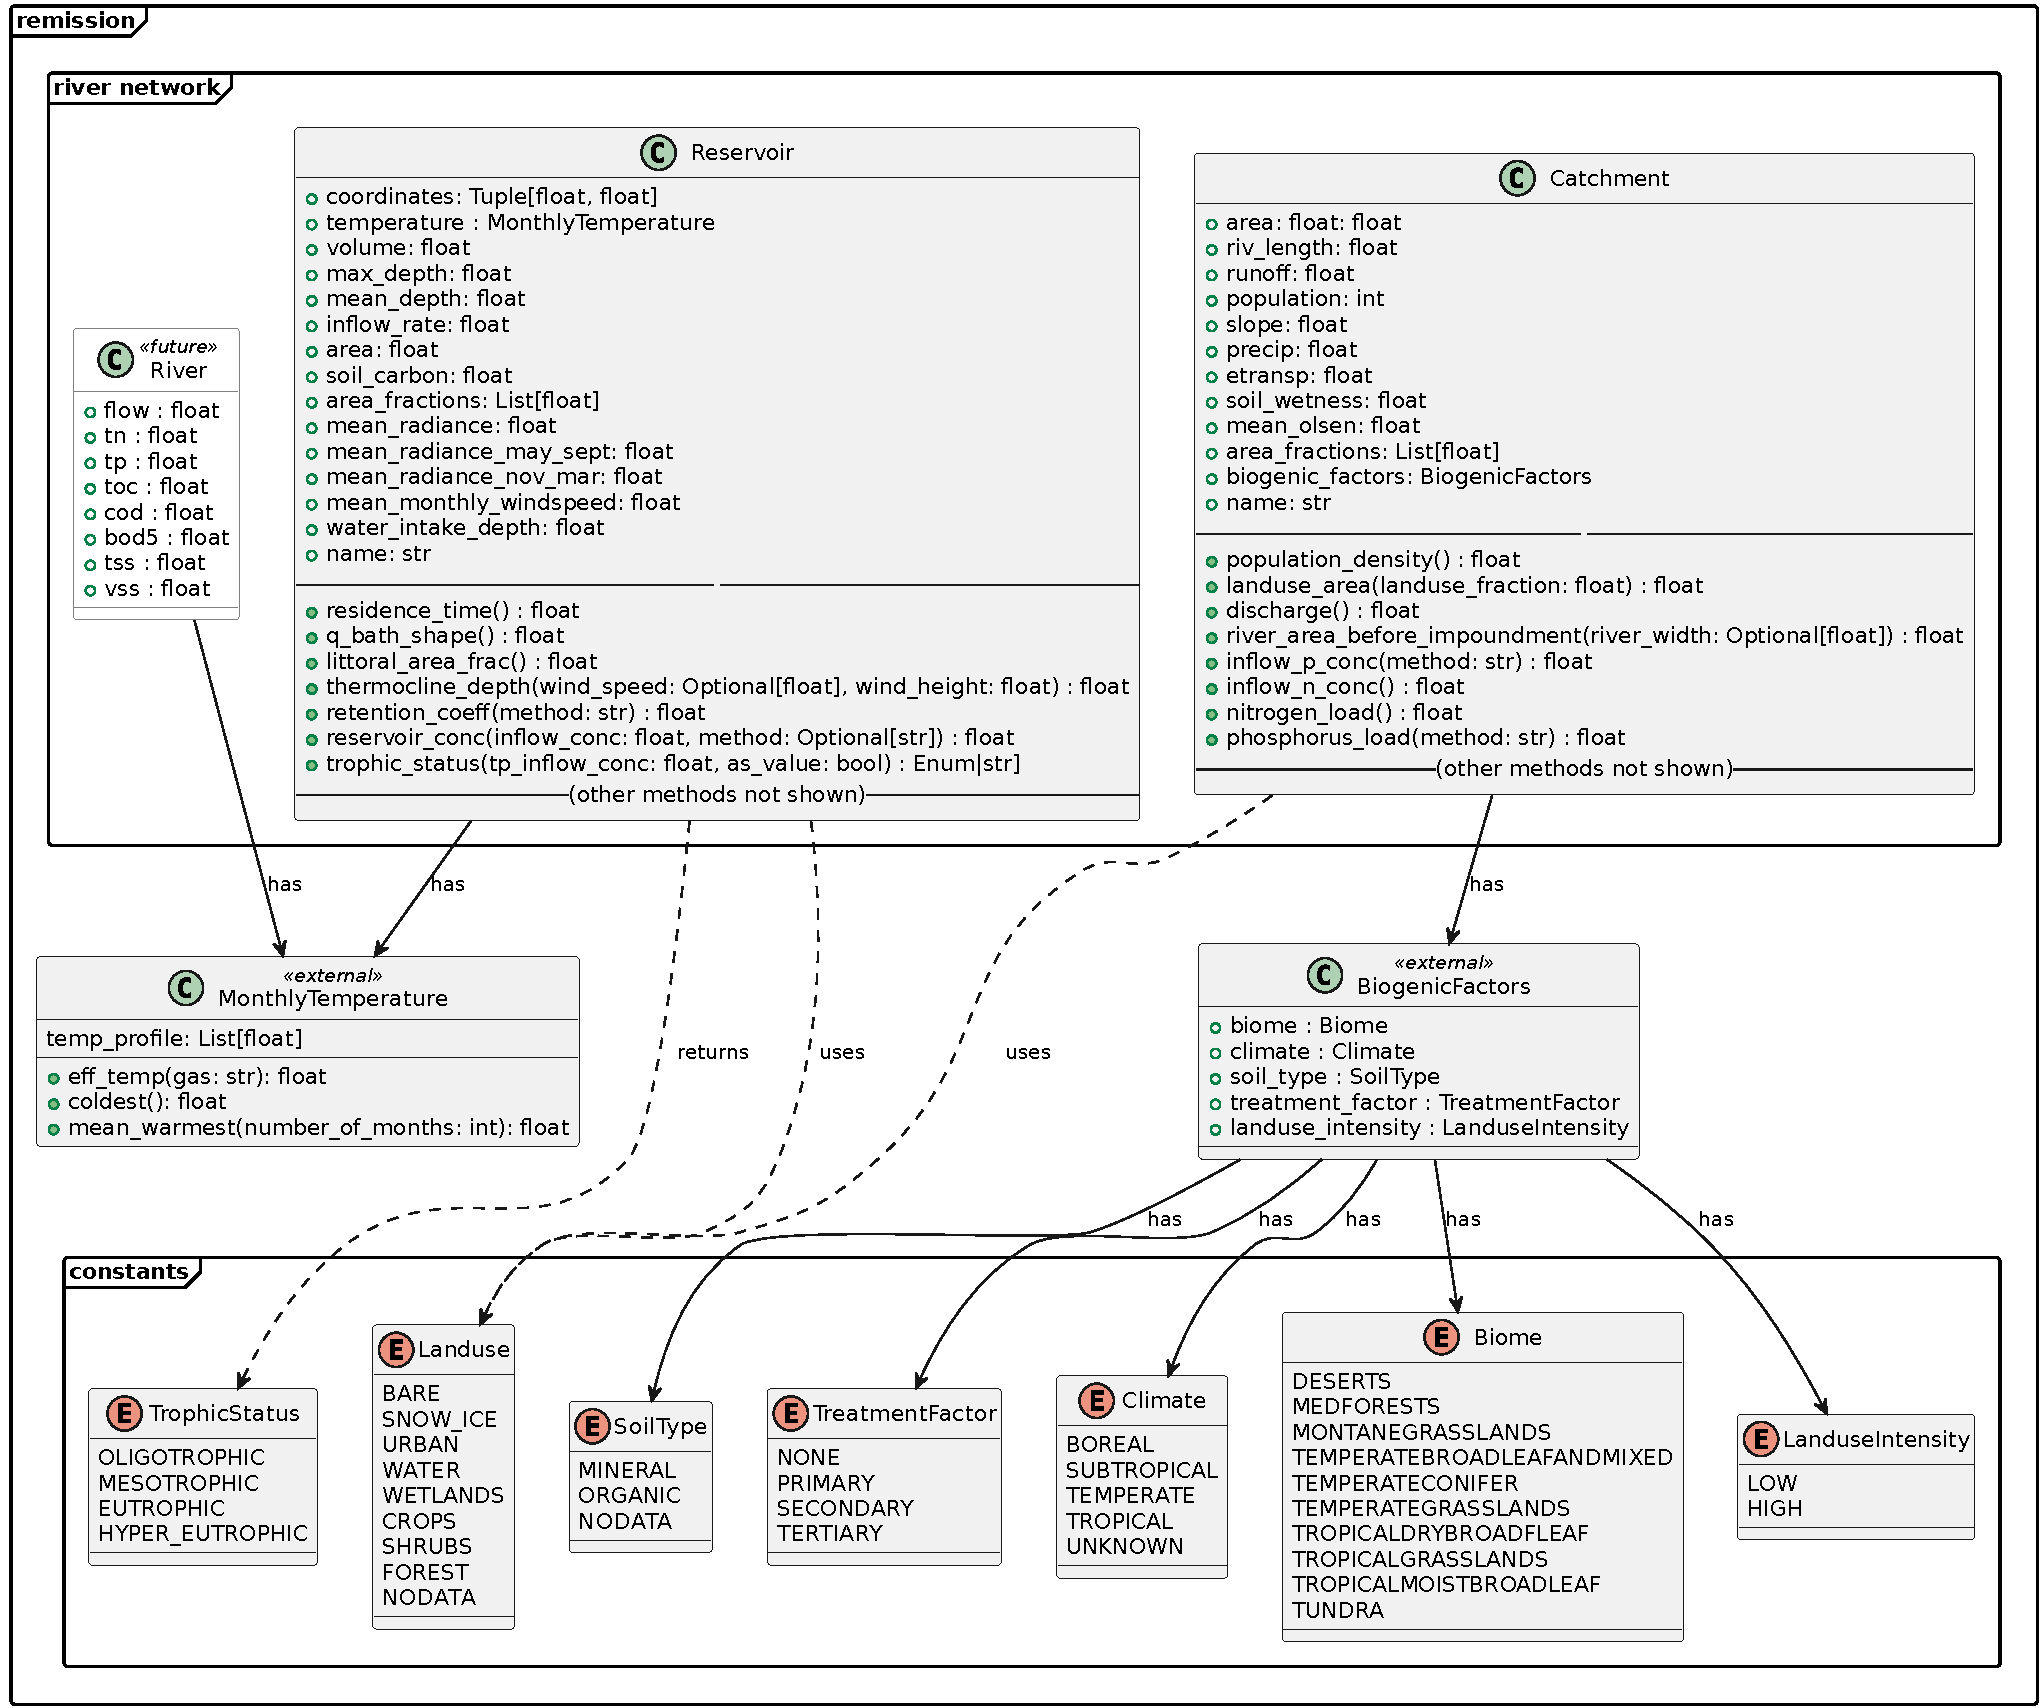
\includegraphics[width=0.99\textwidth]{figures/river_network_uml.pdf}
    \caption{A UML class diagram visualizing the \vrbbrk{Reservoir} and \vrbbrk{Catchment} classes and different container classes and categorical data representations using Enum classes.}
    \label{fig:river_network_emissions_uml}
\end{figure}

\begin{figure}[ht]
    \centering
    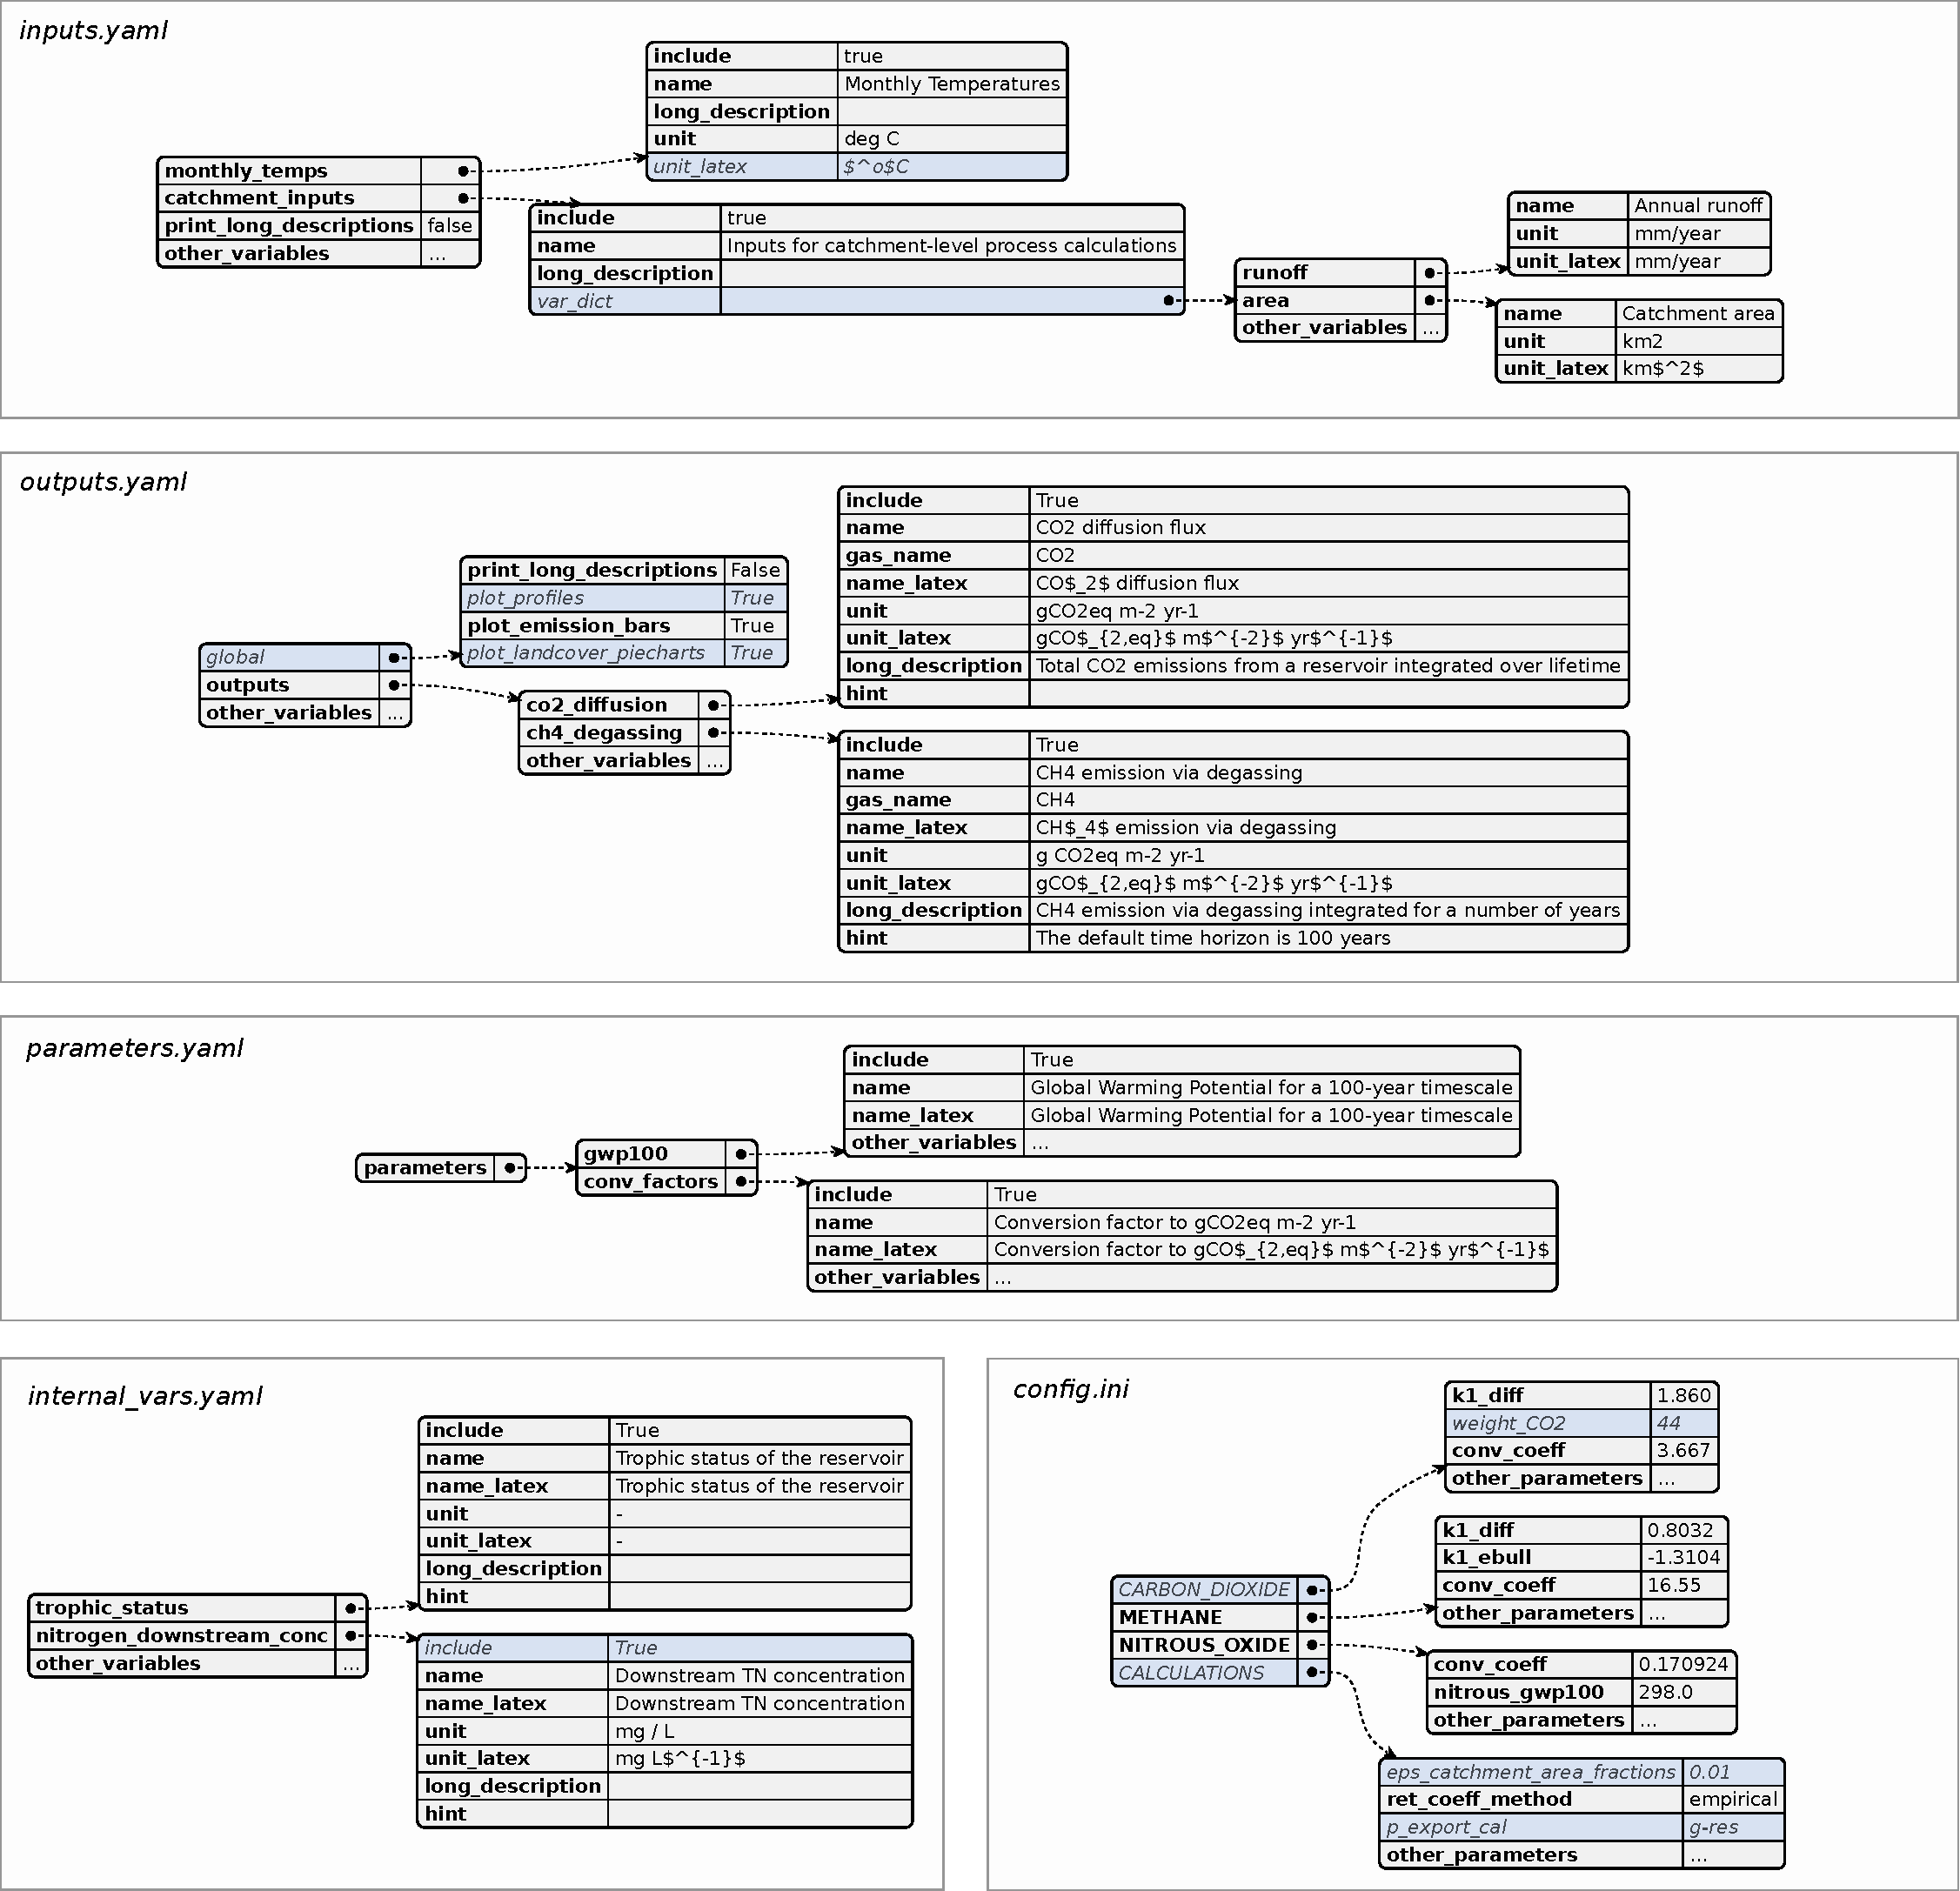
\includegraphics[width=0.99\textwidth]{figures/config_uml_portrait.pdf}
    \caption{Diagrams illustrating the structure of YAML configuration files used by the Presenter class (\vrbbrk{inputs.yaml}, \vrbbrk{outputs.yaml}, \vrbbrk{parameters.yaml}, \vrbbrk{internal\_vars.yaml}), along with the \vrbbrk{config.ini} file specifying emission model parameters and selection of alternative models.}
    \label{fig:config_uml}
\end{figure}

\begin{figure}[ht]
    \centering
    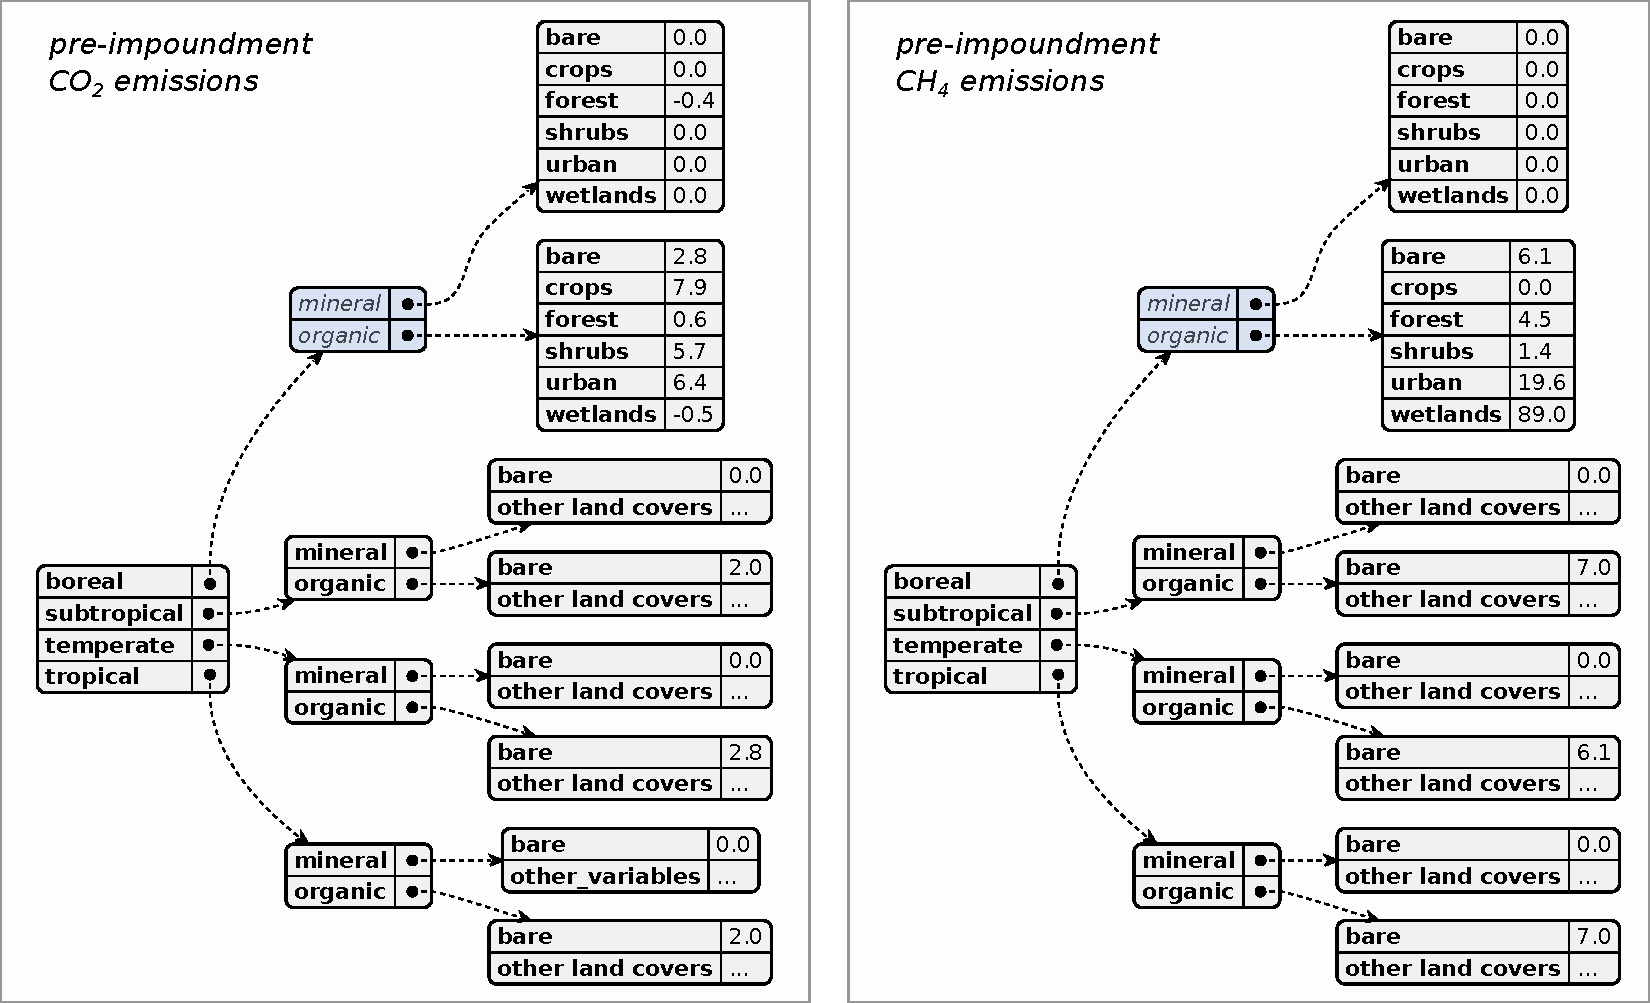
\includegraphics[width=0.80\textwidth]{figures/preimpoundment.pdf}
    \caption{Diagrams illustrating the structure of YAML configuration files and the underlying data relating areal pre-impoundment CO$_2$ and CH$_4$ emissions to climate, soil type, and land cover type.}
    \label{fig:preimpoundment}
\end{figure}

\begin{figure}[ht]
    \centering
    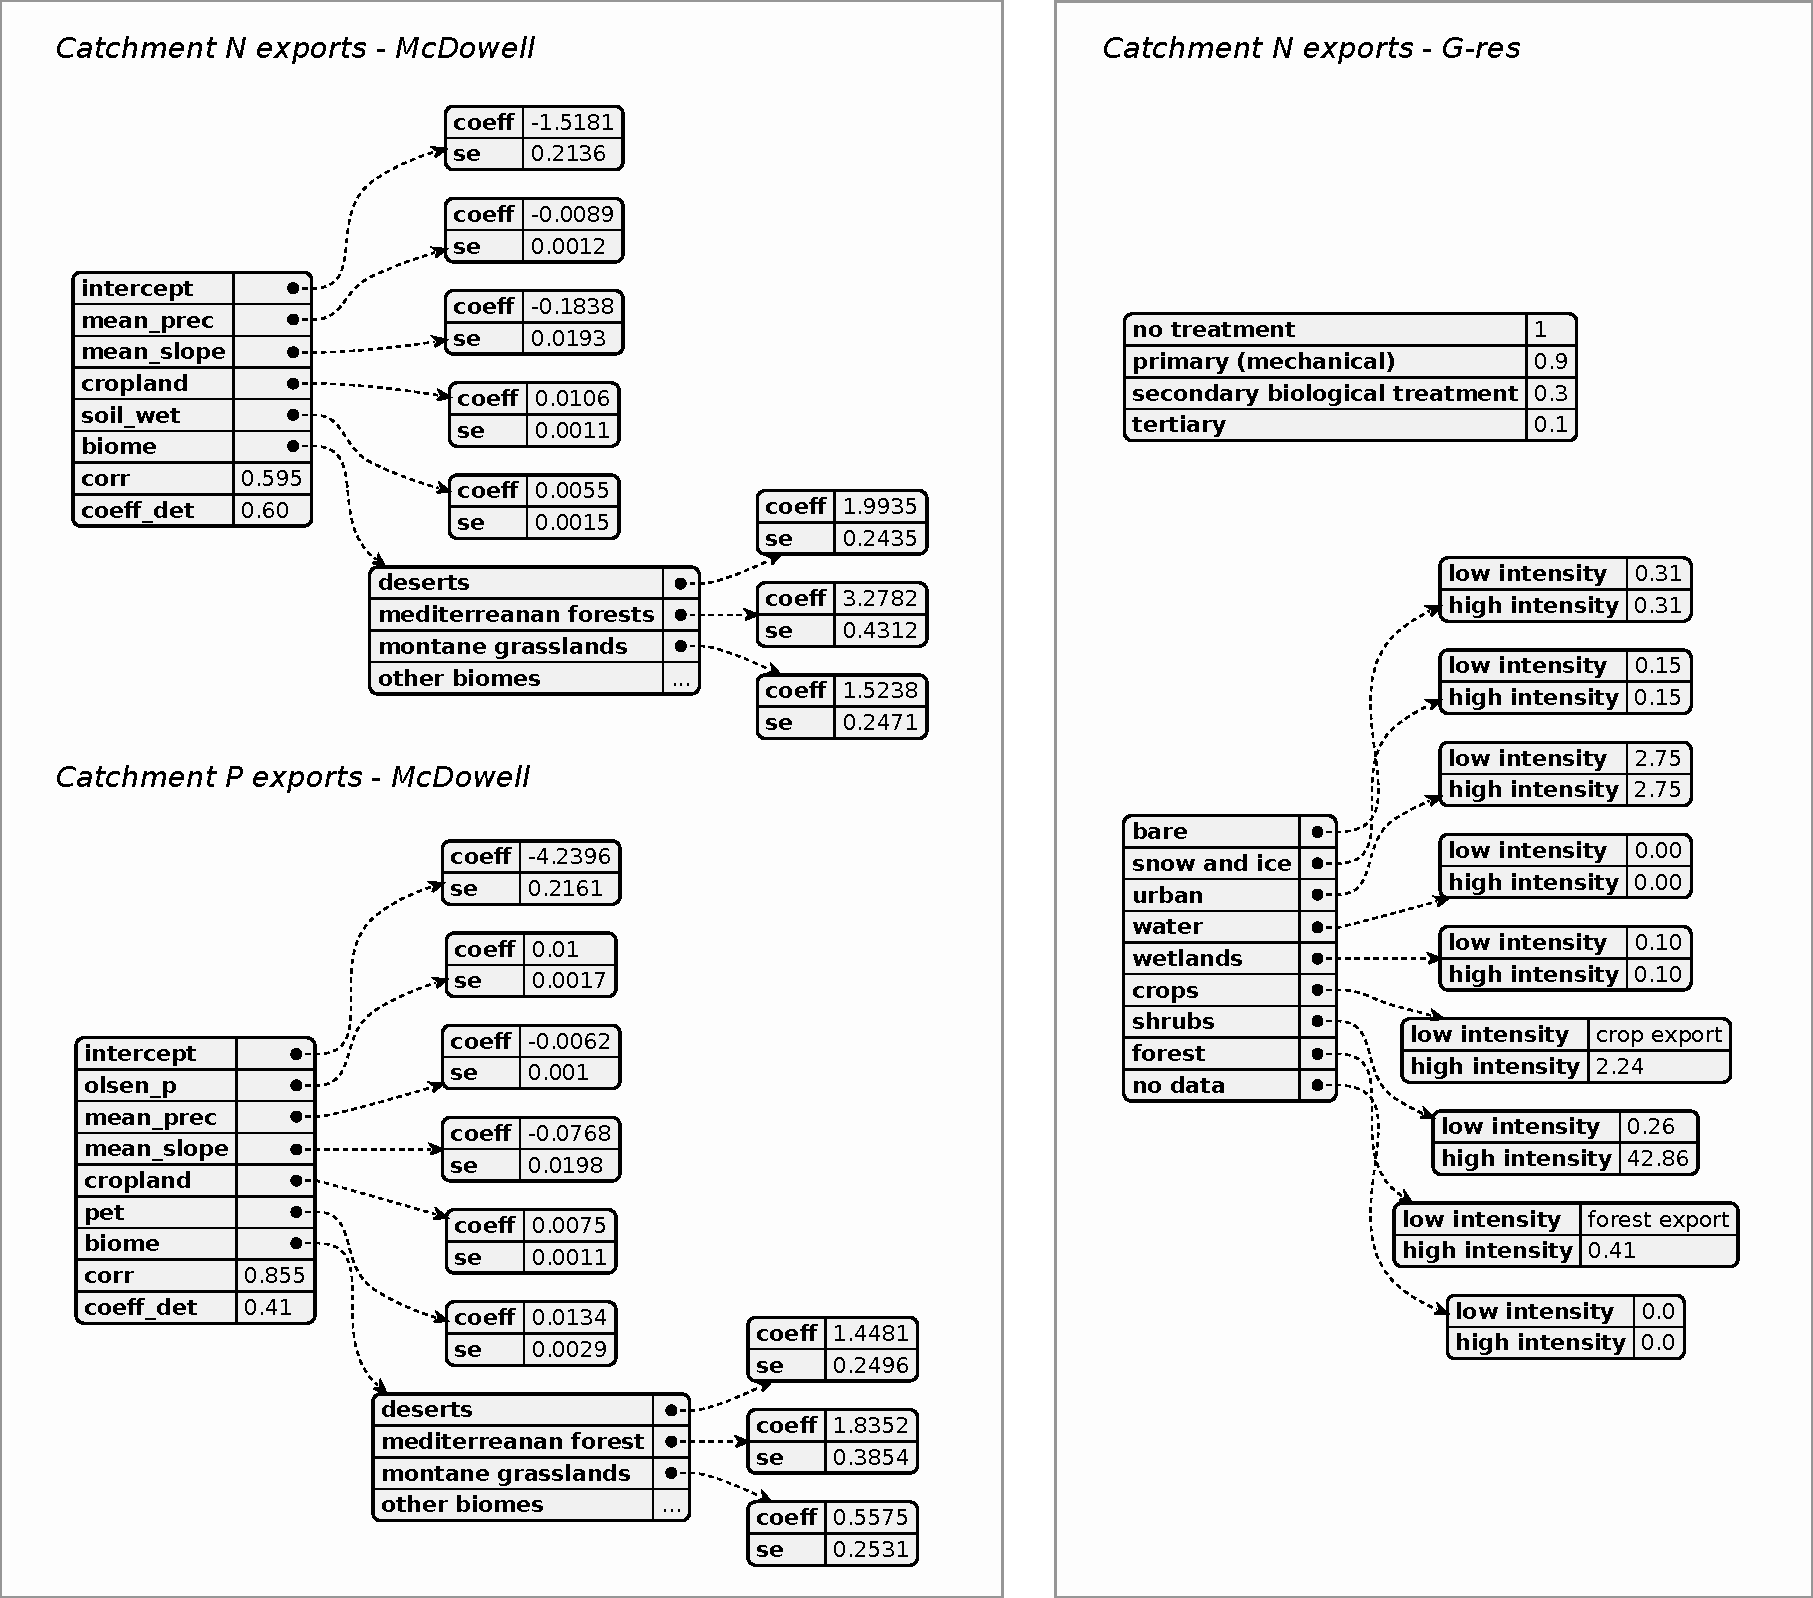
\includegraphics[width=0.85\textwidth]{figures/tp_tn_exports.pdf}
    \caption{Diagrams illustrating the structure of YAML configuration files parameterizing the nutrient export models of \citet{McDowell2020} (\ac{N} and \ac{P}) and G-res (\ac{N}).}
    \label{fig:tp_tn_exports}
\end{figure}

\begin{table}[ht]
	\small
    \caption{Input variables used by Re-Emission for estimating \ac{GHG} emissions from reservoirs}
    \label{app_table:input_variables}%
    \begin{tabular*}{\linewidth}{@{\extracolsep{\fill}}lc@{}}
    \toprule
    Input Name & Unit \\
    \midrule%
    \multicolumn{2}{c}{Inputs for catchment{-}level calculations}\\%
    %\midrule%
    Biome&{-} \\%
    Climate&{-} \\%
    Soil Type&{-} \\%
    Treatment Factor&{-}\\%
    Landuse Intensity&{-}\\%
    Monthly Temperatures&$^o$C\\%
    Annual runoff&mm/year\\%
    Catchment area&km$^2$\\%
    Length of inundated river&km\\%
    Population&capita\\%
    Area fractions\footnotemark[1]&--\\%
    Mean catchment slope&\%\\%
    Mean annual precipitation&mm/year\\%
    Mean annual evapotranspiration&mm/year\\%
    Soil wetness&mm over profile\\%
    Soil Olsen P content&kgP ha$^{-1}$\\%
    \midrule%
    \multicolumn{2}{c}{Inputs for reservoir{-}level calculations}\\%
    %\midrule%
    Reservoir volume&m$^3$\\%
    Reservoir area&km$^2$\\%
    Maximum reservoir depth&m\\%
    Mean reservoir depth&m\\%
    Inundated area fractions\footnotemark[1]&-\\%
    Soil carbon in inundated area&kgC m$^{-2}$\\%
    Mean monthly horizontal radiance&kWh m$^{-2}$ d$^{-1}$\\%
    Mean monthly horizontal radiance: May {-} Sept&kWh m$^{-2}$ d$^{-1}$\\%
    Mean monthly horizontal radiance: Nov {-} Mar&kWh m$^{-2}$ d$^{-1}$\\%
    Mean monthly wind speed&m s$^{-1}$\\%
    Water intake depth below surface&m\\
    \bottomrule
    \end{tabular*}
    \footnotetext[1]{Fractions of land cover in the delineated area.}
    \label{reemission_table}
\end{table}

%\FloatBarrier

\begin{acronym}
	\acro{ASEAN}{Association of Southeast Asian Nations}
	\acro{BRT}{Boosted Regression Tree}
	\acro{CO2}[CO$_2$]{carbon dioxide}
	\acro{CH4}[CH$_4$]{methane}
	\acro{CI}{continuous integration}
	%\acro{CI}{carbon intensity}
	\acro{CLI}{command line interface}
	\acro{DEM}{digital elevation model}
	\acro{DOC}{dissolved organic carbon}
	\acro{DOF}{degree of fragmentation}
	\acro{DOR}{degree of regulation}
	\acro{EF}{emission factor}
	\acro{EFDC}{Environmental Fluid Dynamics Code}
	\acro{EI}{emission intensity}
	\acro{EPA}{U.S. Environmental Protection Agency}
	\acro{ET}{evapotranspiration}
	\acro{FHReD}{High-Resolution Global Database of Dams}
	\acro{FSL}{full supply level}
	\acro{GDrive}{Google Drive}
	\acro{GGRP}{Greenhouse Gas Reporting Program}
	\acro{GEE}{Google Earth Engine}
	\acro{GHCR}{GitHub Container Registry}
    \acro{GHG}{greenhouse gas}    
	\acro{GIS}{geographical information system}
	\acro{G-res}{GHG Reservoir Tool}
	\acro{GOOD2}{Global geOreferenced Database of Dams}
	\acro{GW}{gigawatts}
	\acro{HP}{hydropower}
	\acro{ICOLD}{International Commission on Large Dams}
	\acro{IHA}{International Hydropower Association}
	\acro{KDE}{kernel density estimate}
	\acro{IPCC}{Intergovernmental Panel on Climate Change}
	\acro{KNN}{K-Nearest Neighbours Regressor}
	\acro{LCA}{life-cycle assessment}
	\acro{ML}{machine-learning}
	\acro{MW}{megawatts}
	\acro{MOEA}{multiobjective evolutionary algorithm}
	\acro{MOO}{multiobjective optimization}
	\acro{N}{Nitrogen}
	\acro{N2O}[N$_2$O]{nitrous oxide}
	\acro{P}{Phosphorus}
	\acro{PD}{partial-dependence}
	\acro{PPA}{power purchase agreement}
	\acro{PV}{Photovoltaic}
	\acro{RF}{Random Forest}
	\acro{ROI}{region of interest}
	\acro{RoR}{run-of-river}
	\acro{RMSE}{root-mean-square-error}
	\acro{SA}{sensitivity analysis}
	\acro{SDG}{sustainable development goal}
	\acro{SES}{social and ecological system}
	\acro{SVR}{Support Vector Regression}
	\acro{xAI}{explainable artificial-intelligence}
	\acro{TN}{Total Nitrogen}
	\acro{TP}{Total Phosphorus}
	\acro{UAS}{Unrelated Anthropogenic Sources}
    \acro{VRE}{variable renewable energy}
	\acro{WEFE}{Water-Energy-Food-Ecosystems}
	\acro{WRT}{water residence time}
\end{acronym}

\bibliographystyle{unsrtnat}
\bibliography{reemission}

\end{document}

\endinput
%%
%% End of file `elsarticle-template-num.tex'.
